% !TeX root = RJwrapper.tex
\title{cnefetools: Access and Analysis of Brazilian CNEFE Address Data in R}


\author{by Jorge Ubirajara Pedreira Junior and Bruno Henrique Mioto Stabile}

\maketitle

\abstract{%
The cnefetools package provides programmatic access to the Brazilian National Address File for Statistical Purposes (CNEFE), a geocoded register from the 2022 census, published by the Instituto Brasileiro de Geografia e Estatística (IBGE), with 111.1 million records, one for each type of use found at an address. Although the CNEFE enables fine-grained spatial analyses central to urban and regional planning, such as characterising land use patterns and redistributing census aggregates to arbitrary spatial zones, leveraging it requires overcoming both access barriers, arising from its distribution across thousands of municipality-level files with no unified programmatic interface, and computational barriers from spatial operations that scale to millions of records. cnefetools addresses both through four capabilities: (i) downloading and caching CNEFE data for any of Brazil's 5,570 municipalities; (ii) aggregating address counts to H3 hexagonal grids or user-supplied polygons; (iii) computing land use mix indices; and (iv) performing dasymetric interpolation of census tract variables to arbitrary spatial units using CNEFE dwelling points as ancillary data. The package provides a flexible dual-backend architecture for all computationally intensive operations. The default DuckDB backend reads the cached data in-process and handles all spatial joins, H3 indexing, and aggregations without transferring intermediate results to R, with an advantage that grows with dataset size and exceeds fifteenfold on São Paulo, the largest municipality in the country, where its peak memory is also more than twelve times smaller than the pure-R fallback's.
}

\section{Introduction}\label{introduction}

Address-level data are a fundamental resource for urban and regional
analysis. They enable fine-grained characterisation of land use,
population distribution, and the spatial organisation of economic and
social activities. Unlike parcel boundaries or building footprints,
which often require proprietary sources, geocoded address registers are
administrative by-products of census enumeration, making them publicly
available in several countries.

Brazil is home to the fifth-largest population in the world, with
approximately 213 million inhabitants spread across 5,570 municipalities
\citep{ibge2026}. Since the 2010 Brazilian Census, the \emph{Instituto
Brasileiro de Geografia e Estatística} (IBGE) has produced a rich
by-product: the \emph{Cadastro Nacional de Endereços para Fins Estatísticos}
(CNEFE, National Address File for Statistical Purposes). This dataset
records the geocoordinates and functional category of addresses across
the entire country, in 111.1 million records.

Despite its potential, the CNEFE presents significant barriers to use.
The data are distributed as individual ZIP-compressed CSV files (one per
municipality or state) via the IBGE FTP server. Municipal files can
reach 177 MB compressed (901 MB uncompressed), as in the case of São
Paulo, which contains approximately 5.7 million point addresses. Spatial
operations on these files (assigning points to grid cells, computing
land use mix, or matching them to census tract polygons) require
substantial data engineering. As a result, researchers who could benefit
from this dataset are often unable to leverage it without considerable
ad-hoc effort.

The \CRANpkg{cnefetools} package addresses this gap. It provides a
unified interface for downloading, caching, and analysing CNEFE data
directly from R, with four principal capabilities:

\begin{enumerate}
\def\labelenumi{\arabic{enumi}.}
\tightlist
\item
  \textbf{Data access}: download and read CNEFE data for any municipality,
  with transparent caching to avoid repeated downloads.
\item
  \textbf{Address counts}: aggregate address points to H3 hexagonal grids
  (Uber's open-source hierarchical geospatial indexing system) or
  user-supplied polygons, returning counts by address type.
\item
  \textbf{Land use mix indices}: compute a suite of established and
  novel land use mix (LUM) indices.
\item
  \textbf{Dasymetric interpolation}: redistribute census tract aggregates
  to any spatial unit using CNEFE dwelling points as ancillary data.
\end{enumerate}

For the interpolation task, a few packages exist for this purpose, but
with limitations worth noting. Areal-weighted approaches, such as those
provided by \CRANpkg{sf} \citep{pebesma2018} and \CRANpkg{areal}
\citep{prener2019}, assume a uniform distribution of the attribute within
each source zone, which is methodologically weaker than dasymetric
methods that incorporate ancillary data on where people actually live.
\CRANpkg{populR} \citep{batsaris2023} takes a dasymetric approach using
building footprints as ancillary data. Its volume-weighting mode
additionally incorporates building height or floor counts, but these
remain imperfect proxies: two buildings of equal height may house very
different numbers of households depending on floor plan and unit size,
and height or floor data from volunteered geographic information are
frequently incomplete.

Because each private household record in the CNEFE is one dwelling, the
count of such points within a zone directly reflects the number of
dwellings, making it a more precise
ancillary variable for identifying population density in verticalized
urban environments. Beyond interpolation, no R package currently
provides tools for computing land use mix indices from either
address-level or polygon-based data.

A key technical contribution is a dual-backend architecture. The default
DuckDB backend \citep{duckdb2019}, supported by the \pkg{duckdb} R package,
reads the cached gzipped CSV directly, without prior extraction and
without any third-party extension, performs H3 cell assignment and
spatial joins entirely in-process, and returns only the final aggregated
result to R. Measured against a pure-R fallback based on
\CRANpkg{h3jsr} \citep{h3jsr2023} and \CRANpkg{sf} \citep{pebesma2018}, its
advantage grows with dataset size and exceeds fifteenfold on São Paulo,
where its peak memory is also more than twelve times smaller (see
Section 5 for benchmarks).

This paper is organised as follows. Section 2 describes the CNEFE
dataset and its distribution. Section 3 presents the architectural
decisions underpinning \CRANpkg{cnefetools}. Section 4 describes each
exported function in detail. Section 5 reports performance benchmarks.
Section 6 summarises contributions and discusses future directions.

\section{The CNEFE dataset}\label{the-cnefe-dataset}

The \emph{Cadastro Nacional de Endereços para Fins Estatísticos} (CNEFE) is the
geocoded address register produced alongside the Brazilian Census.
Its production process began in 2005, and it was designed to serve
statistical (rather than postal) purposes, recording not only residences
but also non-residential address points including commercial
establishments, agricultural units, schools, health facilities, and
religious temples \citep{ibge_cnefe2024}. The first CNEFE was published
alongside the 2010 census, though the precision achieved at that time
was limited to the block-face level \citep{ibge_cnefe2024}.
\CRANpkg{cnefetools} therefore targets the 2022 edition
and future censuses, as 2022 is the first to provide address-level
geocoordinates for the full national register.

During the 2022 census, coordinates were collected by enumerators
equipped with mobile devices integrating GNSS receivers. Each device was
preloaded with a list of addresses for the assigned census tract and up
to three GNSS readings were required before the enumerator could
classify an address by functional type. After field collection, IBGE
applied an extensive post-processing workflow: invalid or missing
coordinates were estimated from block-face geometry, confirmed nearby
addresses, or the enumerator's recorded position at the time of
interview. Quality levels were classified by geocoding resolution:
address, block face, locality, or census tract. Pre-census testing
measured mean squared error (MSE) of 5.84 m, with maximum error below
11.71 m under ideal open-sky conditions and typical collection
environments \citep{ibge_cnefe2024}.

\subsection{Structure, scale and distribution}\label{structure-scale-and-distribution}

Each CNEFE record corresponds to one type of use at an address, which
IBGE calls an address species, so an address that hosts more than one
use appears as more than one record
and the number of records exceeds the number of addresses
\citep{ibge_cnefe2024}. In the rest of this paper, \emph{address} refers to a
CNEFE record. The dataset uses a fixed schema of 34 columns. The most analytically relevant
columns are:

\begin{itemize}
\tightlist
\item
  \textbf{\texttt{LONGITUDE}} and \textbf{\texttt{LATITUDE}}: geographic coordinates in the
  SIRGAS 2000 datum (EPSG:4674, approximately equivalent to WGS 84 for
  most applications).
\item
  \textbf{\texttt{COD\_ESPECIE}}: an integer code (1--8) identifying the functional
  category of the address, referred to in this paper as the \emph{address
  type}. The eight categories are listed in Table
  \ref{tab:tab-especie}.
\item
  Address description fields, including street type
  (\textbf{\texttt{NOM\_TIPO\_SEGLOGR}}), street name (\textbf{\texttt{NOM\_SEGLOGR}}), address
  number (\textbf{\texttt{NUM\_ENDERECO}}), free-text address description
  (\textbf{\texttt{DSC\_ESTABELECIMENTO}}), and postal code (\textbf{\texttt{CEP}}).
\end{itemize}

\begin{longtable}[]{@{}
  >{\centering\arraybackslash}p{(\linewidth - 4\tabcolsep) * \real{0.0822}}
  >{\centering\arraybackslash}p{(\linewidth - 4\tabcolsep) * \real{0.3836}}
  >{\centering\arraybackslash}p{(\linewidth - 4\tabcolsep) * \real{0.5342}}@{}}
\caption{\label{tab:tab-especie} CNEFE address types (\protect\texttt{COD\_ESPECIE}).}\tabularnewline
\toprule\noalign{}
\begin{minipage}[b]{\linewidth}\centering
Code
\end{minipage} & \begin{minipage}[b]{\linewidth}\centering
English label
\end{minipage} & \begin{minipage}[b]{\linewidth}\centering
Portuguese label
\end{minipage} \\
\midrule\noalign{}
\endfirsthead
\toprule\noalign{}
\begin{minipage}[b]{\linewidth}\centering
Code
\end{minipage} & \begin{minipage}[b]{\linewidth}\centering
English label
\end{minipage} & \begin{minipage}[b]{\linewidth}\centering
Portuguese label
\end{minipage} \\
\midrule\noalign{}
\endhead
\bottomrule\noalign{}
\endlastfoot
1 & Private household & Domicílio particular \\
2 & Collective household & Domicílio coletivo \\
3 & Agricultural establishment & Estabelecimento agropecuário \\
4 & Educational establishment & Estabelecimento de ensino \\
5 & Health establishment & Estabelecimento de saúde \\
6 & Other establishment & Estabelecimento de outras finalidades \\
7 & Under construction & Edificação em construção ou reforma \\
8 & Religious establishment & Estabelecimento religioso \\
\end{longtable}

The CNEFE covers all 5,570 Brazilian municipalities, with address
counts ranging from a few hundred in small rural municipalities to
approximately 5.7 million in São Paulo, the most populous city in the
Southern
Hemisphere. The consolidated dataset
comprises 111.1 million geographic records, of which 98.95\% were
validated as spatially coherent. More than 110.7 million records
(99.68\%) were geocoded at the address level: 93.8\% from original field
coordinates, 5.5\% with standardised corrections (e.g., apartment units
sharing the same street number), and 0.7\% estimated via spatial
interpolation.

Within the universe of constructed addresses, private dwellings (address
type 1) are the most numerous, comprising approximately 90.6 million
records (81.5\% of the total). Collective households (address type 2)
account for roughly 104,500 records (0.1\%). Among non-residential types,
other-purpose establishments (address type 6) number approximately 11.7
million (10.5\%), followed by agricultural establishments (address type
3) at 4.1 million (3.7\%), while educational (address type 4), health
(address type 5), and religious establishments (address type 8) jointly
account for approximately 1.1 million records (1.0\%). Buildings under
construction (address type 7) numbered approximately 3.5 million (3.2\%).

The data are distributed by IBGE via an FTP server at
\url{https://ftp.ibge.gov.br/Cadastro_Nacional_de_Enderecos_para_Fins_Estatisticos/}.
Files are organised hierarchically by Federative Unit/state (UF) and
municipality. Each municipality's data are stored as a
semicolon-delimited CSV file compressed inside a ZIP archive.

\subsection{Challenges for programmatic use}\label{challenges-for-programmatic-use}

Working with the CNEFE presents several practical difficulties that
\CRANpkg{cnefetools} is designed to overcome:

\begin{itemize}
\item
  \textbf{Discovery}: there is no unified index of download URLs.
  Constructing the correct URL requires knowledge of the state
  acronym, the full municipality name as it appears in the FTP
  directory (which does not always match standard IBGE name fields),
  and the municipality code.
\item
  \textbf{Download size}: while most files are modest, the largest cities
  produce ZIP files running into the hundreds of megabytes.
\item
  \textbf{Spatial operations at scale}: assigning millions of point
  coordinates to hexagonal cells or performing point-in-polygon joins
  with census tract geometries is computationally intensive in pure R.
\end{itemize}

\section{Package design}\label{package-design}

\CRANpkg{cnefetools} addresses the challenges above through three key design
decisions: a pre-built URL index, a persistent user-level cache, and a
dual DuckDB/R backend. The analytical functions --- \texttt{cnefe\_counts()},
\texttt{compute\_lumi()}, \texttt{tracts\_to\_h3()}, and \texttt{tracts\_to\_polygon()} --- each
follow a common two-phase workflow: retrieving the CNEFE data for the
requested municipality (by downloading the ZIP from the IBGE FTP server,
or reading it from a local cache on subsequent calls), and then performing
the requested computation over potentially millions of address records.
\texttt{read\_cnefe()} covers only the first phase, returning the raw CNEFE table
or a spatial object without further aggregation. Because every function
handles retrieval internally, users call whichever function fits their
need directly, without a separate data-loading step. All user-facing
functions additionally validate their inputs with \CRANpkg{checkmate}
\citep{lang2017} before any I/O (normalizing municipality codes, verifying
geometry types, and repairing invalid geometries), so errors are caught
before any network or disk operation begins. Every function works on one
municipality at a time, and Section 6 discusses how analyses that span
several municipalities can be carried out today.

\subsection{Pre-built municipality index}\label{pre-built-municipality-index}

The package ships with an internal data frame (\texttt{cnefe\_index}) that maps
each of Brazil's 5,570 seven-digit IBGE municipality codes to its
corresponding CNEFE ZIP download URL. This index was constructed from
the FTP directory listing at the time of package release. The index also
records the municipality name and the UF, enabling
informative error messages when an unrecognised code is provided.
Municipality codes are validated and normalized by an internal helper,
which accepts integer, character, and numeric inputs and checks that the
code is a seven-digit IBGE code present in the index.

Because the index is fixed when the package is released, it does not
follow later changes to the FTP layout. Before downloading, the package
therefore checks whether the server can be reached and whether the file
exists. An unreachable server points the user to their connection. When
the file is missing, the package lists the published directory, where
file names start with the municipality code, and retries with the URL it
finds there. Only if that also fails does it report that the layout has
changed upstream and ask the user to report it. Either way, a ZIP
obtained by other means can still be read with \texttt{read\_cnefe(file\ =\ ...)},
described below.

\subsection{Persistent user-level caching}\label{persistent-user-level-caching}

Because CNEFE files can be as large as 177 MB compressed for São Paulo,
repeated downloads would impose a
substantial cost on iterative workflows. \CRANpkg{cnefetools} therefore
caches each municipality locally on first download, creating the cache
directory on first use and persisting it across R sessions.

What is cached is a gzipped CSV rather than the ZIP as published. The
conversion runs once, on first download, streamed in chunks so that peak
memory does not scale with the file, and written through a temporary
name so that an interrupted run cannot leave behind something that later
passes for a valid cache entry. Gzip was chosen over raw CSV because it
costs essentially nothing on disk relative to the published ZIP, whereas
the uncompressed CSV is several times larger, and because DuckDB
decompresses it natively, which keeps the read path free of any
third-party extension.

The cache location resolves from the most specific source to the least:
the \texttt{cache\_dir} argument of the calling function, then the
\texttt{CNEFETOOLS\_CACHE\_DIR} environment variable, and finally
\texttt{tools::R\_user\_dir("cnefetools",\ "cache")}, which remains the default so
that users who do nothing see the previous behaviour. Both mechanisms
are offered deliberately, since an environment variable suits a machine
configured once while an explicit argument lets a single call be
redirected without touching the session. The argument is accepted by
every function that reads data, and also by \texttt{clear\_cache\_muni()} and
\texttt{clear\_cache\_tracts()}, because a redirected cache the cleaners could
not see would report success while deleting nothing.

Download integrity is verified by checking that the downloaded file is a
valid ZIP archive and that it contains a CSV file matching the expected
naming pattern. Corrupted or incomplete downloads are detected and
retried with increasing timeout thresholds (300 s, 600 s, and 1,800 s).
Caching can be disabled with \texttt{cache\ =\ FALSE}, in which case the data is
written to a temporary file and removed when the function exits. Users
also have direct control over the local cache: \texttt{clear\_cache\_muni()} and
\texttt{clear\_cache\_tracts()} allow selectively removing cached files, either
all at once or filtered by municipality or state (see Section 4.5).

For workflows that need the data outside this transient cache,
\texttt{cnefe\_export()} writes a permanent copy to a location of the user's
choosing, and the \texttt{file} argument of \texttt{read\_cnefe()} reads such a copy
back without any download (see Section 4.5). Together they let a user
keep an optimised copy on whichever disk suits them, and they also make
ingestion independent of the download path, which matters if access to
the upstream server ever changes.

\subsection{Dual-backend architecture}\label{dual-backend-architecture}

For the computationally intensive operations in \texttt{cnefe\_counts()} and
\texttt{compute\_lumi()}, such as assigning millions of coordinates to H3
hexagons or user-supplied polygons and performing spatial joins, users
can choose between two backends via the \texttt{backend} argument:

\begin{itemize}
\item
  \textbf{\texttt{"duckdb"} (default)}: uses the \CRANpkg{duckdb} \citep{duckdb_r2024}
  R package alongside some DuckDB extensions to spin up an in-memory DuckDB database.
  Reading the cached gzipped CSV requires no extension at all, since
  DuckDB decompresses gzip natively. For H3 aggregation, the \texttt{h3}
  extension assigns cell indices entirely in SQL, while for
  user-provided polygons, the \texttt{spatial} extension and the
  \CRANpkg{duckspatial} R package \citep{duckspatial2026} handle the
  point-in-polygon join.
  Only the final aggregated result is transferred to R. The \texttt{zipfs}
  extension is still available but is loaded on demand, only when the
  file at hand is actually a ZIP, which now happens solely for a cache
  written by an earlier version or for a file the user supplies
  directly.
\item
  \textbf{\texttt{"r"}}: for H3 aggregation, \CRANpkg{h3jsr} assigns each point to
  a cell, whereas for user-provided polygons, \CRANpkg{sf} performs
  the point-in-polygon join. This backend is slower but requires no
  DuckDB dependency whatsoever.
\end{itemize}

The dasymetric interpolation functions \texttt{tracts\_to\_h3()} and
\texttt{tracts\_to\_polygon()} do not expose this argument and rely on DuckDB
exclusively by design, because their cost is dominated by a
point-in-polygon overlay between every dwelling point in the
municipality and the census tract polygons, which is a different and
heavier workload than the tabular aggregation that the pure-R backend
handles, and it is the step that benefits most from DuckDB's spatial
index (Section 4.4).

The census tract geometry assets required by \texttt{tracts\_to\_h3()} and
\texttt{tracts\_to\_polygon()} are stored as Parquet files (one per UF, each
containing a \texttt{geom\_wkb} column with the geometries of census tract
polygons encoded in Well-Known Binary) and published as assets on the
package's GitHub Releases page. They are downloaded on-demand with
caching via the \CRANpkg{piggyback} package \citep{piggyback2023}.

\subsection{Data provenance}\label{data-provenance}

Besides the CNEFE files, which are downloaded from IBGE as published,
the package depends on two data products of its own, the municipality
index and the census tract assets. The scripts that build both are in
the \texttt{data-raw/} directory of the package repository, so either can be
rebuilt or audited.

The index is built by \texttt{data-raw/cnefe\_index\_2022.R}, which takes the
list of 2022 municipalities from \CRANpkg{geobr} and the file names from
the directory listing of each state on the IBGE FTP server.

The census tract assets are built by \texttt{data-raw/sc\_assets\_build.R}. Tract
geometries come from \CRANpkg{geobr}, and tract attributes come from
\CRANpkg{censobr} \citep{pereira2026censobr}, which repackages the IBGE census tract
aggregates, so the variable codes listed in Table
\ref{tab:tab-tracts-vars} are those used by \CRANpkg{censobr}. Some
tracts are returned by \CRANpkg{geobr} as several rows, one for each
disjoint part, and the script dissolves them into a single geometry per
tract, since otherwise the dwelling points of such a tract would be
counted once for each part. The assets for the 2022 edition are served
from the release tag \texttt{sc-assets-v3}, which was built with this script,
and a tract-by-tract comparison with the files originally published
with the package found the same 468,097 tracts in all 27 states and
identical values in all 3,144,868 comparisons. The SHA-256 checksum and size of each
file are recorded in \texttt{data-raw/sc\_assets\_checksums.csv}, so a user can
confirm that a downloaded file is the one that was published.

\section{Core functionality}\label{core-functionality}

The following subsections document each function's interface and
illustrate its use with worked examples. All code examples use address
data for the municipality of Lauro de Freitas, Bahia (IBGE code
2919207).

\subsection{\texorpdfstring{Reading CNEFE data: \texttt{read\_cnefe()}}{Reading CNEFE data: read\_cnefe()}}\label{reading-cnefe-data-read_cnefe}

\texttt{read\_cnefe()} is the entry point to the package. It downloads (if not
cached) and reads the CNEFE CSV for a municipality, returning either an
\CRANpkg{arrow} \citep{arrow2026} \texttt{Table} or an \CRANpkg{sf} point object. The code below
illustrates both output modes for Lauro de Freitas.

\begin{verbatim}
library(cnefetools)

# Read as an Arrow table (default; no spatial conversion)
cnefe <- read_cnefe(
  code_muni = 2919207,
  year      = 2022,
  cache     = TRUE,
  verbose   = TRUE,
  output    = 'arrow'    # default
)

# Read as an sf point object with SIRGAS 2000 coordinates (EPSG:4674)
cnefe_sf <- read_cnefe(
  code_muni = 2919207,
  year      = 2022,
  cache     = TRUE,
  verbose   = TRUE,
  output    = 'sf'
) 
\end{verbatim}

The \texttt{output\ =\ "arrow"} default (an \texttt{arrow::Table}) is preferred for
large municipalities because it avoids materialising the full data frame
in memory. The table can be filtered and projected using \CRANpkg{dplyr}
verbs applied to Arrow tables before conversion to a data frame. The
\texttt{output\ =\ "sf"} option converts the Arrow table to a data frame, coerces
\texttt{LONGITUDE} and \texttt{LATITUDE} to numeric, drops rows with missing
coordinates, and constructs an \texttt{sf} point object in CRS 4674 (SIRGAS
2000).

The code below previews seven selected columns for the first six records
of the dataset previously read as an \texttt{arrow::Table}.

\begin{verbatim}
library(dplyr)

cnefe |>
  select(NOM_TIPO_SEGLOGR, NOM_SEGLOGR, CEP, COD_ESPECIE,
         LONGITUDE, LATITUDE, DSC_ESTABELECIMENTO) |>
  collect() |> 
  head()
#> # A tibble: 6 x 7
#>   NOM_TIPO_SEGLOGR NOM_SEGLOGR           CEP COD_ESPECIE LONGITUDE LATITUDE
#>   <chr>            <chr>               <int>       <int>     <dbl>    <dbl>
#> 1 CAMINHO          31A              42717210           6     -38.3    -12.9
#> 2 RUA              ANILTON DA COSTA 42738440           1     -38.3    -12.9
#> 3 RUA              ANILTON DA COSTA 42738440           7     -38.3    -12.9
#> 4 TRAVESSA         SEM DENOMINACAO  42718005           1     -38.3    -12.9
#> 5 RUA              DO CARMO         42740530           1     -38.4    -12.9
#> 6 RUA              DO CARMO         42740530           1     -38.3    -12.9
#> # i 1 more variable: DSC_ESTABELECIMENTO <chr>
\end{verbatim}

The function accepts the \texttt{year} argument (currently only 2022 is
supported), \texttt{cache} to control caching, and \texttt{verbose} to toggle
informative progress messages. Figure \ref{fig:fig-read-cnefe} maps the
educational establishment addresses for Lauro de Freitas which was
previously read in \texttt{cnefe\_sf}.

\begin{figure}
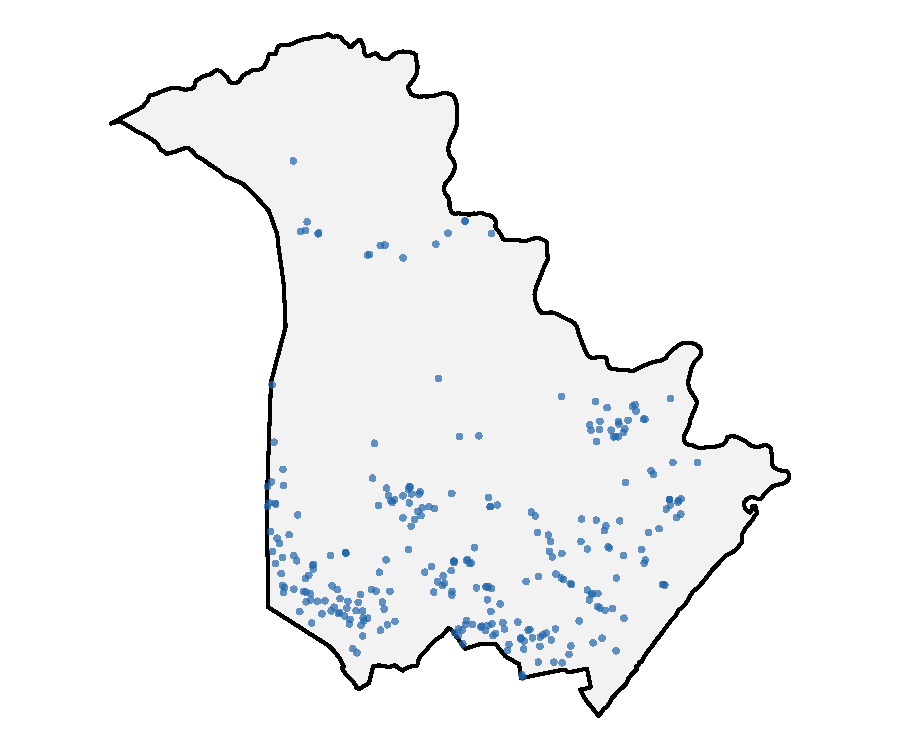
\includegraphics[width=1\linewidth,alt={Map of Lauro de Freitas municipality showing educational establishment address points as blue dots distributed across the urban area, with the municipal boundary outlined in black on a light grey background.}]{cnefetools_files/figure-latex/fig-read-cnefe-1} \caption{Educational establishment addresses geocoded in Lauro de Freitas, Bahia.}\label{fig:fig-read-cnefe}
\end{figure}

\subsection{\texorpdfstring{Address counts on spatial units: \texttt{cnefe\_counts()}}{Address counts on spatial units: cnefe\_counts()}}\label{address-counts-on-spatial-units-cnefe_counts}

\texttt{cnefe\_counts()} aggregates CNEFE address points to areal spatial units
and returns counts of each address type (1 through 8) as columns
\texttt{addr\_type1} to \texttt{addr\_type8}. To illustrate both output modes, the examples
below count addresses per H3 hexagon at resolution 9 and per official
neighborhood boundary obtained from \CRANpkg{geobr} \citep{geobr2019}.

\begin{verbatim}
# Count addresses per H3 hexagon at resolution 9
hex_counts <- cnefe_counts(
  code_muni     = 2919207,
  year          = 2022,
  cache         = TRUE,
  h3_resolution = 9,
  verbose       = TRUE,
  backend       = "duckdb"
)

# Count per user-supplied polygon (e.g., neighborhoods)
library(geobr)
library(dplyr)

nei <- read_neighborhood(year = 2022) |> 
  filter(code_muni == 2919207)

poly_counts <- cnefe_counts(
  code_muni    = 2919207,
  year         = 2022,
  cache        = TRUE,
  polygon      = nei,
  crs_output   = NULL,
  verbose      = TRUE,
  backend      = "duckdb"
)
\end{verbatim}

When no \texttt{polygon} is supplied (the default), the function builds a
complete H3 grid over the municipality boundary using \CRANpkg{geobr} to obtain the
boundary polygon and \CRANpkg{h3jsr} to generate the hexagon geometries.
The DuckDB \texttt{h3} extension is used (when \texttt{backend\ =\ "duckdb"}) to assign
CNEFE points to cells in SQL, but the grid itself is always constructed
via \CRANpkg{h3jsr}. The H3 resolution can be set from 0 (coarse) to 15
(fine), and the default is 9, corresponding to an average hexagon area
of approximately 105,000 m².

That figure is an average, because H3 is not an equal-area grid. Cells
are laid out on an icosahedron projected onto the globe, so cells of the
same resolution differ in area depending on where they fall. Across
Brazil, resolution 9 cells range from about 80,000 m² to 127,000 m², so
the largest is about 1.6 times the smallest. This matters whenever an
analysis assumes cells of equal size, as in density estimates. When
equal area is a requirement, an equal-area grid is the better choice,
such as the A5 grid available in \CRANpkg{a5R} \citep{a5r2026} or IGEO7,
which is built on the ISEA projection \citep{kmoch2025}. \CRANpkg{cnefetools}
uses H3 because the DuckDB \texttt{h3} extension assigns cells inside the
query, which keeps the aggregation in-process, and because H3 cell
identifiers can be joined with other data indexed on the same grid.

When a \texttt{polygon} is supplied, the function performs a point-in-polygon
join between the CNEFE coordinates and the user-supplied \texttt{sf} polygon. A
warning is issued if any CNEFE points fall outside the polygon, together
with the coverage percentage, and an error is raised if no points fall
inside.

The output \texttt{sf} object inherits the polygon geometry: H3 hexagons when
\texttt{polygon} is \texttt{NULL}, or the user-supplied polygons (in their original
CRS, or \texttt{crs\_output} if specified) when one is given. Figure
\ref{fig:fig-counts} illustrates both modes for Lauro de Freitas at H3
resolution 8 and at the neighborhood level.

\begin{figure}
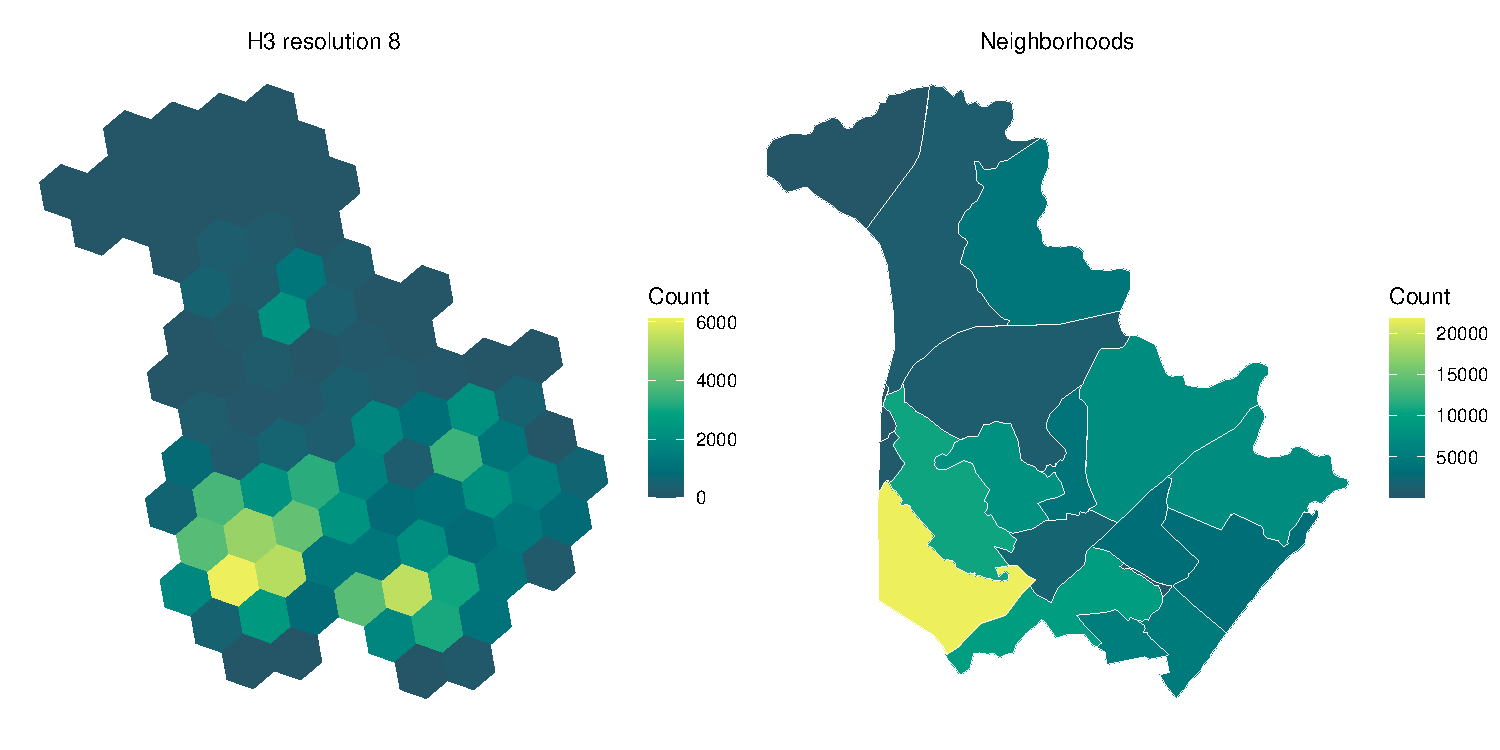
\includegraphics[width=1\linewidth,alt={Two side-by-side choropleth maps of Lauro de Freitas. The left map shows private household address counts aggregated to H3 hexagons at resolution 8; the right map shows the same counts aggregated to neighborhoods. Both maps use a green-to-yellow colour scale where darker green indicates lower counts and bright yellow indicates higher counts.}]{cnefetools_files/figure-latex/fig-counts-1} \caption{Private household address counts (\texttt{addr\_type1}) aggregated to H3 hexagons at resolution~8 (left) and to neighborhoods (right) for Lauro de Freitas, Bahia.}\label{fig:fig-counts}
\end{figure}

\subsection{\texorpdfstring{Land use mix indices: \texttt{compute\_lumi()}}{Land use mix indices: compute\_lumi()}}\label{land-use-mix-indices-compute_lumi}

\texttt{compute\_lumi()} computes a suite of six land use mix (LUM) indices from
CNEFE address data, providing the first R implementation of this class
of spatial indicators. No other CRAN package implements land use mix
indices, whether from address-level or polygon-based data. All indices
are based on the local residential share
\(p_i = n_{\text{res},i} / n_{\text{tot},i}\), where \(n_{\text{res},i}\) is
the count of type-1 addresses (private households) and
\(n_{\text{tot},i}\) is the total count of addresses of all types except
type 7 (under construction). The citywide residential share \(P\) is
computed in the same way over the whole municipality, and it is used by
the Balance Index and by the BGBI.

Table \ref{tab:lumi-table} summarises the six indices computed by
\texttt{compute\_lumi()}, together with the residential share \(p_i\) on which
they are based, which is also returned. Further methodological details on these indices can be
found in \citet{song2013}, \citet{massey2001}, \citet{pedreirajr2025} and
\citet{pedreirajr2026bgbi}.

\begin{longtable}[]{@{}
  >{\centering\arraybackslash}p{(\linewidth - 6\tabcolsep) * \real{0.2361}}
  >{\centering\arraybackslash}p{(\linewidth - 6\tabcolsep) * \real{0.2361}}
  >{\centering\arraybackslash}p{(\linewidth - 6\tabcolsep) * \real{0.2917}}
  >{\centering\arraybackslash}p{(\linewidth - 6\tabcolsep) * \real{0.2361}}@{}}
\caption{\label{tab:lumi-table} Land use mix indices returned by \protect\texttt{compute\_lumi()}.
Here \(q_i = 1 - p_i\) and \(r = P/(1-P)\).}\tabularnewline
\toprule\noalign{}
\begin{minipage}[b]{\linewidth}\centering
Index
\end{minipage} & \begin{minipage}[b]{\linewidth}\centering
Code
\end{minipage} & \begin{minipage}[b]{\linewidth}\centering
Formula
\end{minipage} & \begin{minipage}[b]{\linewidth}\centering
Range
\end{minipage} \\
\midrule\noalign{}
\endfirsthead
\toprule\noalign{}
\begin{minipage}[b]{\linewidth}\centering
Index
\end{minipage} & \begin{minipage}[b]{\linewidth}\centering
Code
\end{minipage} & \begin{minipage}[b]{\linewidth}\centering
Formula
\end{minipage} & \begin{minipage}[b]{\linewidth}\centering
Range
\end{minipage} \\
\midrule\noalign{}
\endhead
\bottomrule\noalign{}
\endlastfoot
Residential share & \texttt{p\_res} & \(p_i\) & \([0,1]\) \\
Entropy Index & \texttt{ei} & \(-\,(p_i \ln p_i + q_i \ln q_i)\,/\ln 2\) & \([0,1]\) \\
Herfindahl-Hirschman Index & \texttt{hhi} & \(p_i^2 + q_i^2\) & \([0.5,\,1]\) \\
Balance Index & \texttt{bal} & \(1 - \lvert p_i - r\,q_i\rvert\,/\,(p_i + r\,q_i)\) & \([0,1]\) \\
Index of Concentration at Extremes & \texttt{ice} & \(p_i - q_i\) & \([-1,+1]\) \\
Adapted HHI & \texttt{hhi\_adp} & \(\mathrm{sign}(p_i - q_i)\cdot(\mathrm{HHI}_i - 0.5)\,/\,0.5\) & \([-1,+1]\) \\
BGBI & \texttt{bgbi} & \([(2p_i-1)-(2P-1)]\,/\,[1-(2p_i-1)(2P-1)]\) & \([-1,+1]\) \\
\end{longtable}

All the indices therefore rest on a binary split, in which an address
counts as residential only when it is a private household (type 1) and
as non-residential otherwise. They measure the balance between housing
and all other uses, not the diversity of those other uses, so an area
whose non-residential addresses are all of one type scores the same as
an area where they are spread across every type, provided both have the
same residential share. This is the formulation on which the indices
were defined and validated against job accessibility in
\citet{pedreirajr2026bgbi}, but it differs from the multi-category definitions
of land use mix that are common in urban research \citep{song2013}. Users who
need the diversity of non-residential uses can compute it from the
counts by address type that \texttt{cnefe\_counts()} returns.

Type 7 addresses are left out because a building under construction or
renovation describes a transitional state rather than a realised use.
Such buildings are likely to be concentrated where a city is expanding,
so leaving them out makes the indices describe those areas as they are
now rather than as they will be once the buildings are occupied. If
these buildings end up in the same proportions as existing addresses,
among which private households are the large majority, the indices
understate the residential share those areas are heading towards, and
the effect is largest where type 7 makes up a large share of addresses.
\texttt{cnefe\_counts()} does not apply this exclusion and reports these
addresses as \texttt{addr\_type7}, so users can check how many there are in any
area of interest.

Because \(P\) is computed from counts of address types, it describes how
addresses are distributed across types in the municipality, not how
residents are distributed. It is also always computed over the whole
municipality, including when
\texttt{polygon} is supplied, because it is meant to describe the city that
the addresses belong to. A baseline computed only over the area covered
by the polygons would measure mix relative to that area rather than
relative to the city, which is a different quantity.

The parameter interface of \texttt{compute\_lumi()} mirrors that of
\texttt{cnefe\_counts()}:

\begin{verbatim}
# Compute all indices on H3 hexagons at resolution 9 (default)
lumi_hex <- compute_lumi(
  code_muni     = 2919207,
  year          = 2022,
  cache         = TRUE,
  h3_resolution = 9,
  verbose       = TRUE,
  backend       = "duckdb"
)

# Compute on user-supplied polygons
lumi_poly <- compute_lumi(
  code_muni    = 2919207,
  year         = 2022,
  cache        = TRUE,
  polygon      = nei,
  crs_output   = NULL,
  verbose      = TRUE,
  backend      = "duckdb"
)
\end{verbatim}

The output \texttt{sf} object contains columns \texttt{id\_hex} (or the original
polygon columns), \texttt{p\_res}, \texttt{ei}, \texttt{hhi}, \texttt{bal}, \texttt{ice}, \texttt{hhi\_adp}, \texttt{bgbi},
and the polygon geometry. Figure \ref{fig:fig-bgbi} maps the BGBI index
\citep{pedreirajr2026bgbi} for Lauro de Freitas at H3 resolution 8 and at the
neighborhood level.

\begin{figure}
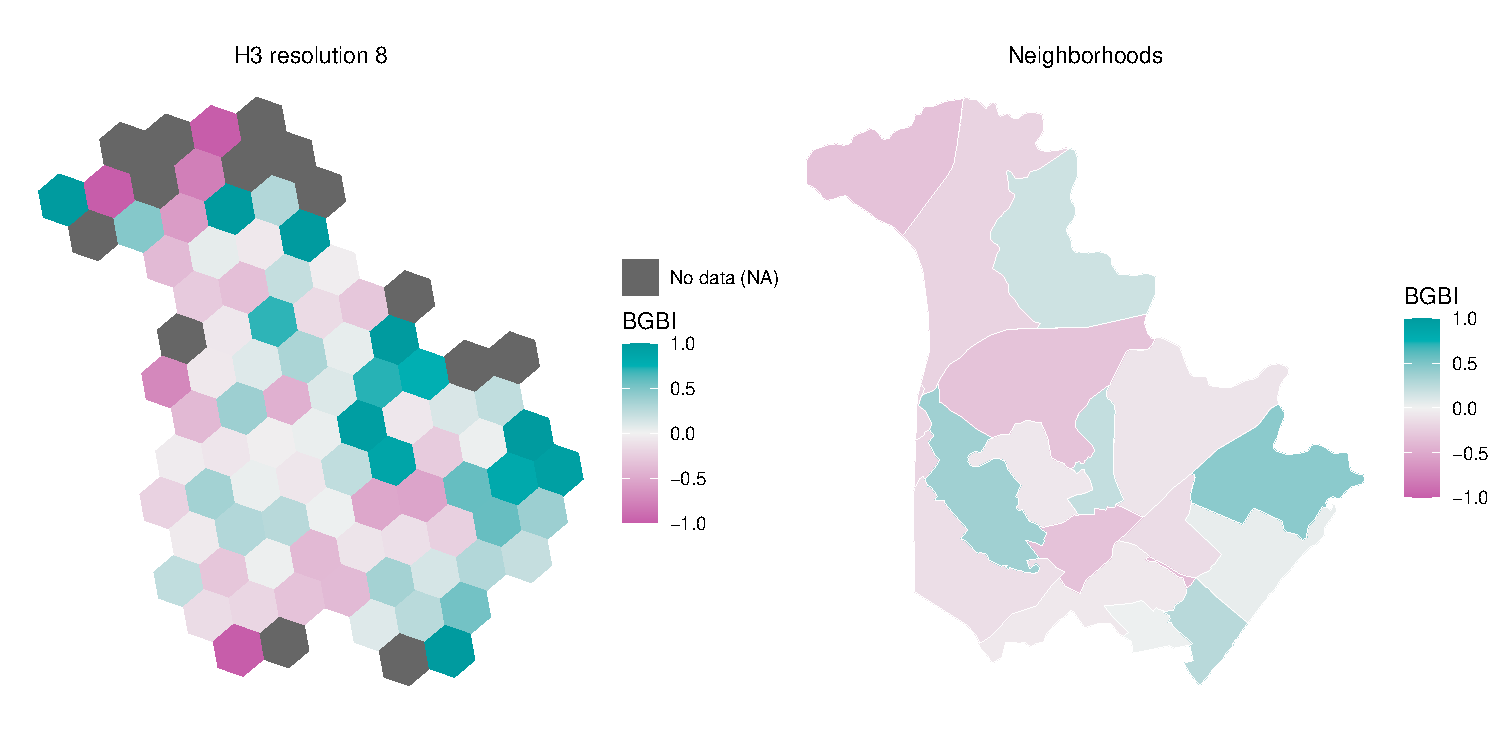
\includegraphics[width=1\linewidth,alt={Two side-by-side choropleth maps of Lauro de Freitas showing the BGBI index. The left map aggregates to H3 hexagons at resolution 8 and the right map aggregates to neighborhoods. Green areas indicate a local residential share above the citywide average, pink areas indicate non-residential dominance, and white or neutral areas are near the citywide baseline.}]{cnefetools_files/figure-latex/fig-bgbi-1} \caption{Bidirectional Global-centered Balance Index (BGBI) for Lauro de Freitas, Bahia, aggregated to H3 hexagons at resolution~8 (left) and to neighborhoods (right). Green cells indicate a local residential share above the citywide average ($p_i > P$); pink cells indicate non-residential dominance ($p_i < P$); white cells are near the citywide baseline.}\label{fig:fig-bgbi}
\end{figure}

Figure \ref{fig:fig-bgbi} illustrates how the spatial pattern of the
BGBI can differ markedly between the H3 hexagonal grid and neighborhood
boundaries: some neighborhoods aggregate areas of contrasting land use,
smoothing out local variation that remains visible at the hexagon level,
while the coarser polygon boundaries may shift which zones appear
residentially dominant or non-residential. By allowing the same indices
to be computed across multiple H3 resolutions and over user-supplied
polygon layers, \CRANpkg{cnefetools} makes it straightforward to assess the
sensitivity of land use mix measurement to spatial aggregation and,
therefore, to explicitly probe scale effects associated with the
Modifiable Areal Unit Problem (MAUP) \citep{dark2007}.

\subsection{\texorpdfstring{Dasymetric interpolation: \texttt{tracts\_to\_h3()} and \texttt{tracts\_to\_polygon()}}{Dasymetric interpolation: tracts\_to\_h3() and tracts\_to\_polygon()}}\label{dasymetric-interpolation-tracts_to_h3-and-tracts_to_polygon}

The 2022 Brazilian Census disseminates questionnaire results through
multiple geographic products, one of which is the \emph{Agregados por Setores
Censitários} (aggregates by census tract). A census tract (\emph{setor
censitário}) is the basic territorial unit of census collection and of
this particular dissemination product. For many applications, however,
the desired spatial unit differs from census tracts, as researchers may
want data on a regular H3 grid for comparative analyses, or on custom
polygons such as traffic zones for transportation modelling or health
districts for public health management. For this purpose,
\CRANpkg{cnefetools} addresses this need with \texttt{tracts\_to\_h3()} and \texttt{tracts\_to\_polygon()},
which perform dasymetric interpolation \citep{mennis2003} from census tract aggregates
to user-defined spatial units using CNEFE dwelling points as ancillary data.

Several R packages tackle this polygon-to-polygon transfer problem using
areal weighting. \CRANpkg{sf} \citep{pebesma2018}, through
\texttt{st\_interpolate\_aw()}, and \CRANpkg{areal} \citep{prener2019}, through
\texttt{aw\_interpolate()}, both distribute source-zone totals in proportion to
the overlap area between source and target polygons, implicitly assuming
a uniform spatial distribution of the attribute within each source zone.

\CRANpkg{smile} \citep{smile2025} addresses the same change-of-support problem through a
model-based approach. Source-zone values are treated as spatial averages
of a latent Gaussian random field, \texttt{fit\_spm()} estimates the field
parameters from the source data, and \texttt{predict\_spm()} aggregates
predicted field values over target polygons or point locations, returning
point estimates alongside prediction uncertainty. The redistribution is driven
entirely by the modelled spatial correlation structure and no ancillary data are
used.

\CRANpkg{populR} \citep{batsaris2023} is the closest in spirit to
\CRANpkg{cnefetools}. The \texttt{pp\_estimate()} function supports both areal
weighting and a dasymetric mapping that uses building footprints as
ancillary data, weighting the redistribution by an estimate of building
volume (derived from footprint area multiplied by building height or
floor count) rather than by plain overlap area. Building
polygons must be supplied by the user from any available source.
\texttt{pp\_compare()} additionally facilitates accuracy assessment against
reference counts.

\CRANpkg{cnefetools} follows the same dasymetric logic as the
volume-weighting mode of \CRANpkg{populR}, but uses geocoded dwelling
points from the CNEFE register instead of building footprints. This
distinction matters in verticalized urban environments, as building
footprints capture ground-floor area but carry no information about how
many dwelling units a building contains. Even when volume is
approximated by multiplying footprint area by building height or floor
count, height alone is an imperfect proxy for dwelling count. Two
buildings of equal height may differ substantially in the number of
households they contain depending on floor plan and unit size.

Although dwelling count is itself an imperfect proxy as the number of
occupants per dwelling varies across households, it is a more defensible
ancillary variable for redistribution than built area or building
height. The variables available for interpolation are listed in Table
\ref{tab:tab-tracts-vars}, alongside their variable code, as used by
\CRANpkg{censobr}, and the census tract table they come from.

\begin{table}

\caption{\label{tab:tab-tracts-vars}Variables supported by \textbackslash{}texttt\{tracts\textbackslash{}\_to\textbackslash{}\_h3()\} and \textbackslash{}texttt\{tracts\textbackslash{}\_to\textbackslash{}\_polygon()\}, with their variable codes and source tables, with codes as used by censobr. Portuguese descriptions are available in \textbackslash{}texttt\{tracts\textbackslash{}\_variables\textbackslash{}\_ref\textbackslash{}\$desc\textbackslash{}\_var\textbackslash{}\_ibge\}.}
\centering
\begin{tabular}[t]{lll}
\toprule
Variable & Variable code & Source table\\
\midrule
pop\_ph & V00005 & Domicilios\\
pop\_ch & V00007 & Domicilios\\
male & V01007 & Pessoas\\
female & V01008 & Pessoas\\
age\_0\_4 & V01031 & Pessoas\\
\addlinespace
age\_5\_9 & V01032 & Pessoas\\
age\_10\_14 & V01033 & Pessoas\\
age\_15\_19 & V01034 & Pessoas\\
age\_20\_24 & V01035 & Pessoas\\
age\_25\_29 & V01036 & Pessoas\\
\addlinespace
age\_30\_39 & V01037 & Pessoas\\
age\_40\_49 & V01038 & Pessoas\\
age\_50\_59 & V01039 & Pessoas\\
age\_60\_69 & V01040 & Pessoas\\
age\_70m & V01041 & Pessoas\\
\addlinespace
race\_branca & V01317 & Pessoas\\
race\_preta & V01318 & Pessoas\\
race\_parda & V01320 & Pessoas\\
race\_amarela & V01319 & Pessoas\\
race\_indigena & V01321 & Pessoas\\
\addlinespace
n\_resp & V06001 & ResponsavelRenda\\
avg\_inc\_resp & V06004 & ResponsavelRenda\\
\bottomrule
\end{tabular}
\end{table}

The entire computation pipeline runs within an in-memory DuckDB instance
and proceeds in six steps, with all heavy operations remaining inside
DuckDB until the final aggregated result is materialised in R, followed
by a diagnostic report:

\begin{enumerate}
\def\labelenumi{\arabic{enumi}.}
\item
  \textbf{DuckDB setup}: an in-memory DuckDB database is opened and the
  \texttt{spatial} extension is loaded for the \texttt{ST\_Within} point-in-polygon
  joins, together with the \texttt{h3} extension for cell assignment in SQL
  in the case of \texttt{tracts\_to\_h3()}. Reading the
  cached data needs no extension, since DuckDB decompresses gzip
  natively.
\item
  \textbf{Census tract geometry}: the UF-level Parquet asset is registered
  as a DuckDB \texttt{VIEW} and immediately materialised into a persistent
  in-memory \texttt{TABLE}. A spatial R-tree index (\texttt{USING\ RTREE}) is built
  on the tract geometry column to accelerate the subsequent
  point-in-polygon join.
\item
  \textbf{CNEFE points}: DuckDB streams the semicolon-delimited CSV
  straight out of the cached gzipped file, without extracting it to
  disk and without an extension to mediate the read. Only
  rows with \texttt{COD\_ESPECIE} \(\in \{1, 2\}\) (private and collective
  dwellings) and non-null coordinates are retained and materialised
  into a second in-memory \texttt{TABLE}.
\item
  \textbf{Spatial join and allocation}: an inner \texttt{ST\_Within} join matches
  each dwelling point to its enclosing census tract. Per-tract counts
  of type-1 (\texttt{n\_dom\_p}) and type-2 (\texttt{n\_dom\_c}) matched points serve as
  denominators. Variable-specific allocation expressions are assembled
  into a single SQL \texttt{VIEW} (\texttt{cnefe\_alloc}) and, for \texttt{tracts\_to\_h3()},
  H3 cell indices are assigned in the same step via
  \texttt{h3\_latlng\_to\_cell\_string(lat,\ lon,\ resolution)}. All intermediate
  results remain inside DuckDB with no transfer to R at this stage.
  Table \ref{tab:tab-alloc} summarises the allocation rule for each
  variable group.
\item
  \textbf{Aggregation}: the \texttt{cnefe\_alloc} view is grouped by target spatial
  unit (H3 cell or polygon identifier). Count variables are aggregated
  with \texttt{SUM}, while \texttt{avg\_inc\_resp} is aggregated with \texttt{AVG} (mean of
  per-point tract averages, weighted implicitly by the number of
  eligible points per cell). This produces a compact result table with
  one row per non-empty target unit.
\item
  \textbf{Materialisation and output}: the aggregated result is pulled into
  R with a single \texttt{dbGetQuery()} call. For \texttt{tracts\_to\_h3()}, the
  complete H3 grid for the municipality is built in R via
  \CRANpkg{h3jsr} (including border hexagons recovered via a \(k = 1\)
  neighbour ring) and joined to the DuckDB result with a \texttt{LEFT\ JOIN},
  so hexagons with no eligible dwelling points are retained with count
  variables set to 0 and \texttt{avg\_inc\_resp} set to \texttt{NA}. For
  \texttt{tracts\_to\_polygon()}, the user-supplied \texttt{sf} polygons are the join
  target.
\end{enumerate}

\begin{table}
\centering
\caption{\label{tab:tab-alloc}Allocation rules applied during dasymetric interpolation. \texttt{n\_dom\_p} and \texttt{n\_dom\_c} are counts of matched type-1 and type-2 CNEFE dwelling points per census tract.}
\centering
\resizebox{\ifdim\width>\linewidth\linewidth\else\width\fi}{!}{
\begin{tabular}[t]{llll}
\toprule
Variable & Eligible type & Per-point value & Aggregated as\\
\midrule
\texttt{pop\_ph} & Type 1 (private) & total / n\_dom\_p & SUM\\
\texttt{pop\_ch} & Type 2 (collective) & total / n\_dom\_c & SUM\\
\texttt{n\_resp} & Type 1 (private) & total / n\_dom\_p & SUM\\
\texttt{male}, \texttt{female}, \texttt{age\_*}, \texttt{race\_*} & Type 1; else Type 2 & total / n\_eligible & SUM\\
\texttt{avg\_inc\_resp} & Type 1 (private) & tract avg (assigned) & MEAN\\
\bottomrule
\end{tabular}}
\end{table}

\begin{enumerate}
\def\labelenumi{\arabic{enumi}.}
\setcounter{enumi}{6}
\tightlist
\item
  \textbf{Diagnostics}: regardless of the \texttt{verbose} setting, the function
  always emits a two-stage diagnostic report. Stage 1 reports, for
  each requested variable, the share of the tract-level total
  successfully allocated to CNEFE points, the number of tracts with
  \texttt{NA} source values, and the number of tracts where no eligible
  dwelling points were found. Stage 2 reports the share of allocated
  CNEFE points that fall within at least one target spatial unit.
\end{enumerate}

\begin{verbatim}
# Interpolate population in private and collective households to H3 hexagons
hex_pop <- tracts_to_h3(
  code_muni     = 2919207,
  h3_resolution = 9,
  vars          = c("pop_ph", "pop_ch"),
  cache         = TRUE,
  verbose       = TRUE
)

# Interpolate to user-supplied polygons (e.g., traffic zones)
poly_pop <- tracts_to_polygon(
  code_muni = 2919207,
  polygon   = nei,                          # Lauro de Freitas' neighborhoods 
  vars      = c("pop_ph", "avg_inc_resp"),
  cache         = TRUE,
  verbose       = TRUE
)
\end{verbatim}

Figure \ref{fig:fig-pop} shows dasymetric estimates of
private-household population (\texttt{pop\_ph}) for Lauro de Freitas at H3
resolution 8 and at the neighborhood level.

\begin{figure}
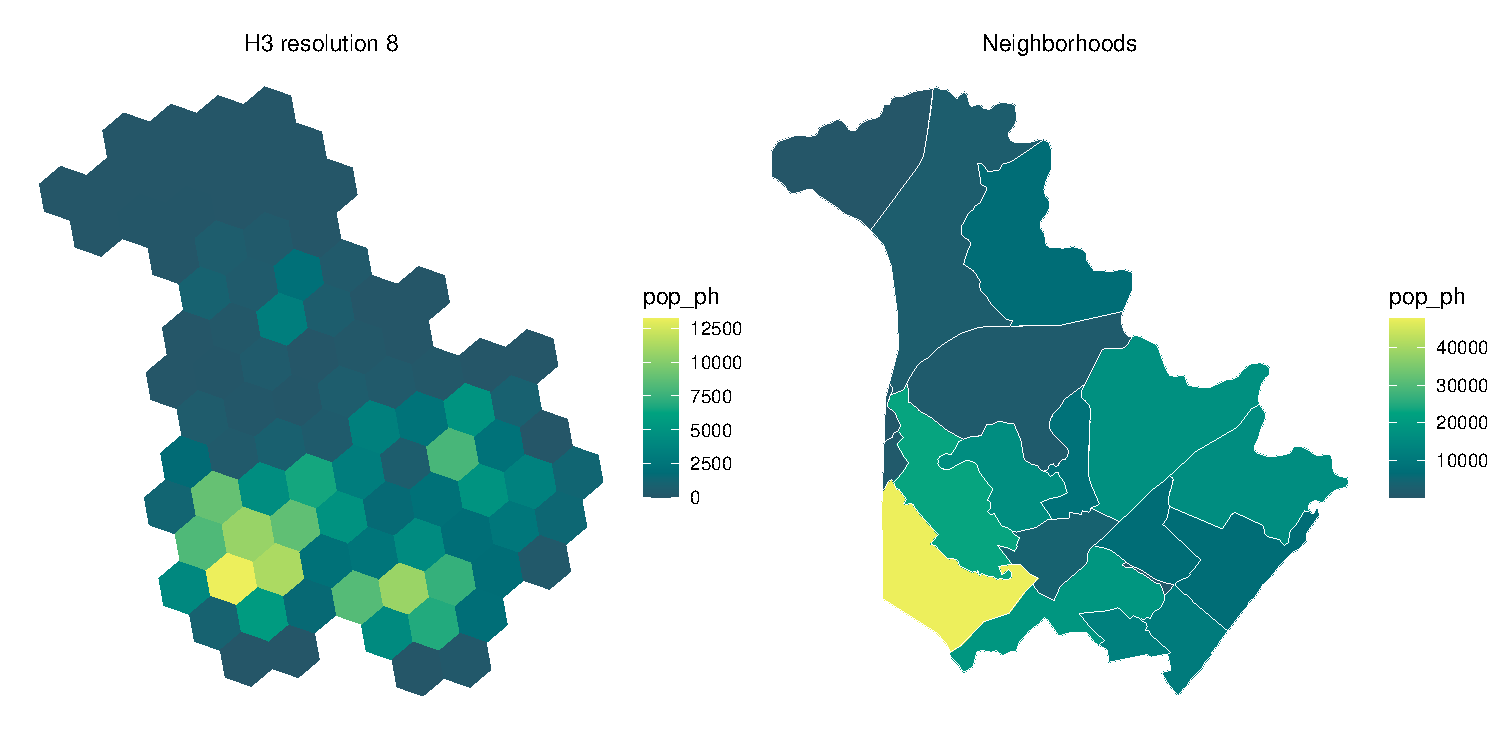
\includegraphics[width=1\linewidth,alt={Two side-by-side choropleth maps of Lauro de Freitas showing dasymetric estimates of private-household population. The left map shows estimates on H3 hexagons at resolution 8 and the right map shows estimates on neighborhoods. Both use a green-to-yellow colour scale where brighter yellow indicates higher population counts.}]{cnefetools_files/figure-latex/fig-pop-1} \caption{Dasymetric estimates of private-household population (\texttt{pop\_ph}) for Lauro de Freitas, Bahia, interpolated from 2022 census tract totals to H3 hexagons at resolution~8 (left) and to neighborhoods (right) using CNEFE dwelling points as ancillary data.}\label{fig:fig-pop}
\end{figure}

The diagnostic summary is displayed at the end of each call, regardless
of the \texttt{verbose} setting. Running \texttt{tracts\_to\_polygon()} for Lauro de
Freitas with \texttt{vars\ =\ c("pop\_ph",\ "avg\_inc\_resp")} produces the following
report:

\begin{verbatim}
poly_diag <- cnefetools::tracts_to_polygon(
  code_muni = 2919207,
  polygon   = nei,
  vars      = c("pop_ph", "avg_inc_resp"),
  verbose   = FALSE
)
#> v spatial extension loaded
#> 
#> -- Dasymetric interpolation diagnostics --
#> 
#> -- Stage 1: Tracts → CNEFE points
#> ! Unallocated total for population from private households (pop_ph): 0 of
#>   202583 (0.00%)
#> ! avg_inc_resp assigned to 95484 of 95515 eligible points (99.97% of total
#>   points)
#> ! avg_inc_resp is NA in 4 of 354 tracts (1.13% of total tracts)
#> ! Unmatched CNEFE points (no tract): 186 of 95739 points (0.19% of total
#>   points)
#> ! Tracts with NA totals: pop_ph in 4 of 354 tracts (1.13% of total tracts).
#> 
#> -- Stage 2: CNEFE points → Polygons
#> i Polygon coverage: 95492 of 95553 allocated points captured (99.94%)
\end{verbatim}

Stage 1 of the report describes how completely the census tract totals
were allocated to CNEFE dwelling points before aggregation to the target
polygons. The unallocated fraction for count variables such as \texttt{pop\_ph}
measures the share of the official population total that could not be
distributed because certain tracts contained no eligible CNEFE dwelling
points in the matched dataset. For \texttt{avg\_inc\_resp}, the diagnostic
additionally reports the number of tracts where the income variable is
\texttt{NA} in the IBGE source table.

Stage 2 describes how well the user-supplied polygons capture the
allocated dwelling points. The coverage percentage is the share of all
allocated CNEFE points that fall within at least one of the provided
polygons. Values below 100\% indicate that some dwelling points lie
outside the polygon layer. Polygons with no captured CNEFE points
receive zero for all count variables and \texttt{NA} for \texttt{avg\_inc\_resp} in the
output object.

Users should bear in mind that dasymetric interpolation produces
estimates, not observed values. The method assumes that the attribute
being redistributed (e.g., population) is distributed proportionally to
dwelling points within each census tract. While this is a more realistic
assumption than uniform areal weighting, it remains an approximation: if
population density varies systematically within a tract in ways not
captured by the CNEFE point pattern, the sub-tract estimates will be
correspondingly biased. Inferences about individuals or households from
these tract-level aggregates are therefore subject to the ecological
fallacy \citep{robinson1950}.

\subsection{Utility functions}\label{utility-functions}

\CRANpkg{cnefetools} also exports five utility functions for documentation
access, cache management and data export. \texttt{cnefe\_dictionary()} opens the official
CNEFE data dictionary (an Excel file bundled with the package) in the
system's default spreadsheet viewer, providing column definitions and
value codes for all 34 fields of the CNEFE schema. \texttt{cnefe\_doc()} opens
the bundled IBGE methodological note \citep{ibge_cnefe2024} as a PDF,
detailing the geocoding procedures and quality classifications used in
the 2022 census.

\begin{verbatim}
cnefe_dictionary()  # opens the Excel data dictionary
cnefe_doc()         # opens the IBGE methodological PDF
\end{verbatim}

\texttt{clear\_cache\_muni()} deletes cached CNEFE files from the cache
directory, either all at once or for a specific municipality identified
by its seven-digit IBGE code. \texttt{clear\_cache\_tracts()} removes cached
census tract Parquet files, with optional filtering by state, accepting
a two-letter UF abbreviation, a two-digit numeric state code, or a
seven-digit municipality code (which is resolved to its state
automatically).

\begin{verbatim}
clear_cache_muni()          # delete all cached CNEFE files
clear_cache_muni(2919207)   # delete only the file for Lauro de Freitas-BA

clear_cache_tracts()        # delete all cached census tract Parquets
clear_cache_tracts("BA")    # delete only the Parquet for the state of Bahia ("BA")
\end{verbatim}

\texttt{cnefe\_export()} writes a municipality to a directory of the user's
choosing as Parquet (the default), CSV or gzipped CSV, so that an
analysis can keep its own copy of the data instead of depending on the
cache, which the functions above are meant to empty. The \texttt{file}
argument of \texttt{read\_cnefe()} reads any of those formats, as well as the
ZIP exactly as IBGE publishes it, and skips the download entirely.

\begin{verbatim}
# Write Lauro de Freitas-BA to a project folder as Parquet
path <- cnefe_export(2919207, path = "data/cnefe")

# Read it back later without downloading anything
cnefe <- read_cnefe(file = path)
\end{verbatim}

\section{Performance}\label{performance}

The DuckDB backend derives its performance advantage from three sources:

\begin{enumerate}
\def\labelenumi{\arabic{enumi}.}
\tightlist
\item
  \textbf{In-process execution}: DuckDB runs as a library within the R
  process, eliminating the overhead of client--server communication.
\item
  \textbf{Streaming aggregation}: DuckDB decompresses the cached gzipped
  CSV natively, with no extension involved, and aggregates as it
  scans, so the full address table is never materialised. For São
  Paulo, this is the difference between holding roughly 5.7 million
  addresses in memory and holding only the running group totals.
\item
  \textbf{Vectorised query execution}: DuckDB uses a columnar engine with
  SIMD-accelerated operations, making aggregation and joins over tens
  of millions of rows substantially faster than row-oriented R
  operations.
\end{enumerate}

Performance is benchmarked along two independent dimensions. The first
varies municipality size (measured by the number of CNEFE address
points) while holding the H3 output resolution fixed at 8, using three
municipalities of increasing size. The second varies H3 resolution
across levels 7, 9, and 11 while holding the municipality fixed at
Curitiba-PR. All measurements were collected on a machine with a
14-core Intel Core i9-13900H (2.60 GHz), 32 GB RAM, Windows 11, R 4.6.0,
and DuckDB 1.5.2.

Elapsed times drift within a session as the CPU changes thermal and
frequency state, by as much as a factor of two, so timing every DuckDB
case and then every pure-R case would load that drift onto one backend
and make it indistinguishable from the effect being measured. Each
configuration is therefore visited once per pass, round-robin, and the
pass is repeated three to five times, with every replicate run in a
fresh R subprocess after a discarded warm-up. The figures report the
median across replicates, and the whiskers show the observed minimum
and maximum. Peak memory is the operating system's peak working set for
the whole R process, obtained through the \texttt{ps} package rather than
R-level allocation tracking, which counts only the R heap and would miss
what DuckDB allocates in C++.
Figure \ref{fig:fig-bench-cities} shows that DuckDB reduces the median
elapsed time for \texttt{cnefe\_counts()} from 4.69 s to 3.79 s for Vitória da
Conquista-BA (approximately 200,000 addresses, 1.24× speedup), from
9.19 s to 3.53 s for Curitiba-PR (approximately 900,000 addresses,
2.60× speedup), and from 93.25 s to 5.58 s for São Paulo-SP
(approximately 5.7 million addresses, 16.7× speedup). The relative
advantage grows with dataset size, because DuckDB's columnar engine and
streaming scan scale more favourably than row-oriented R operations. For
small municipalities, the fixed initialisation overhead of opening a
connection and loading the H3 extension can dominate and the two
backends perform comparably.

\begin{figure}

{\centering 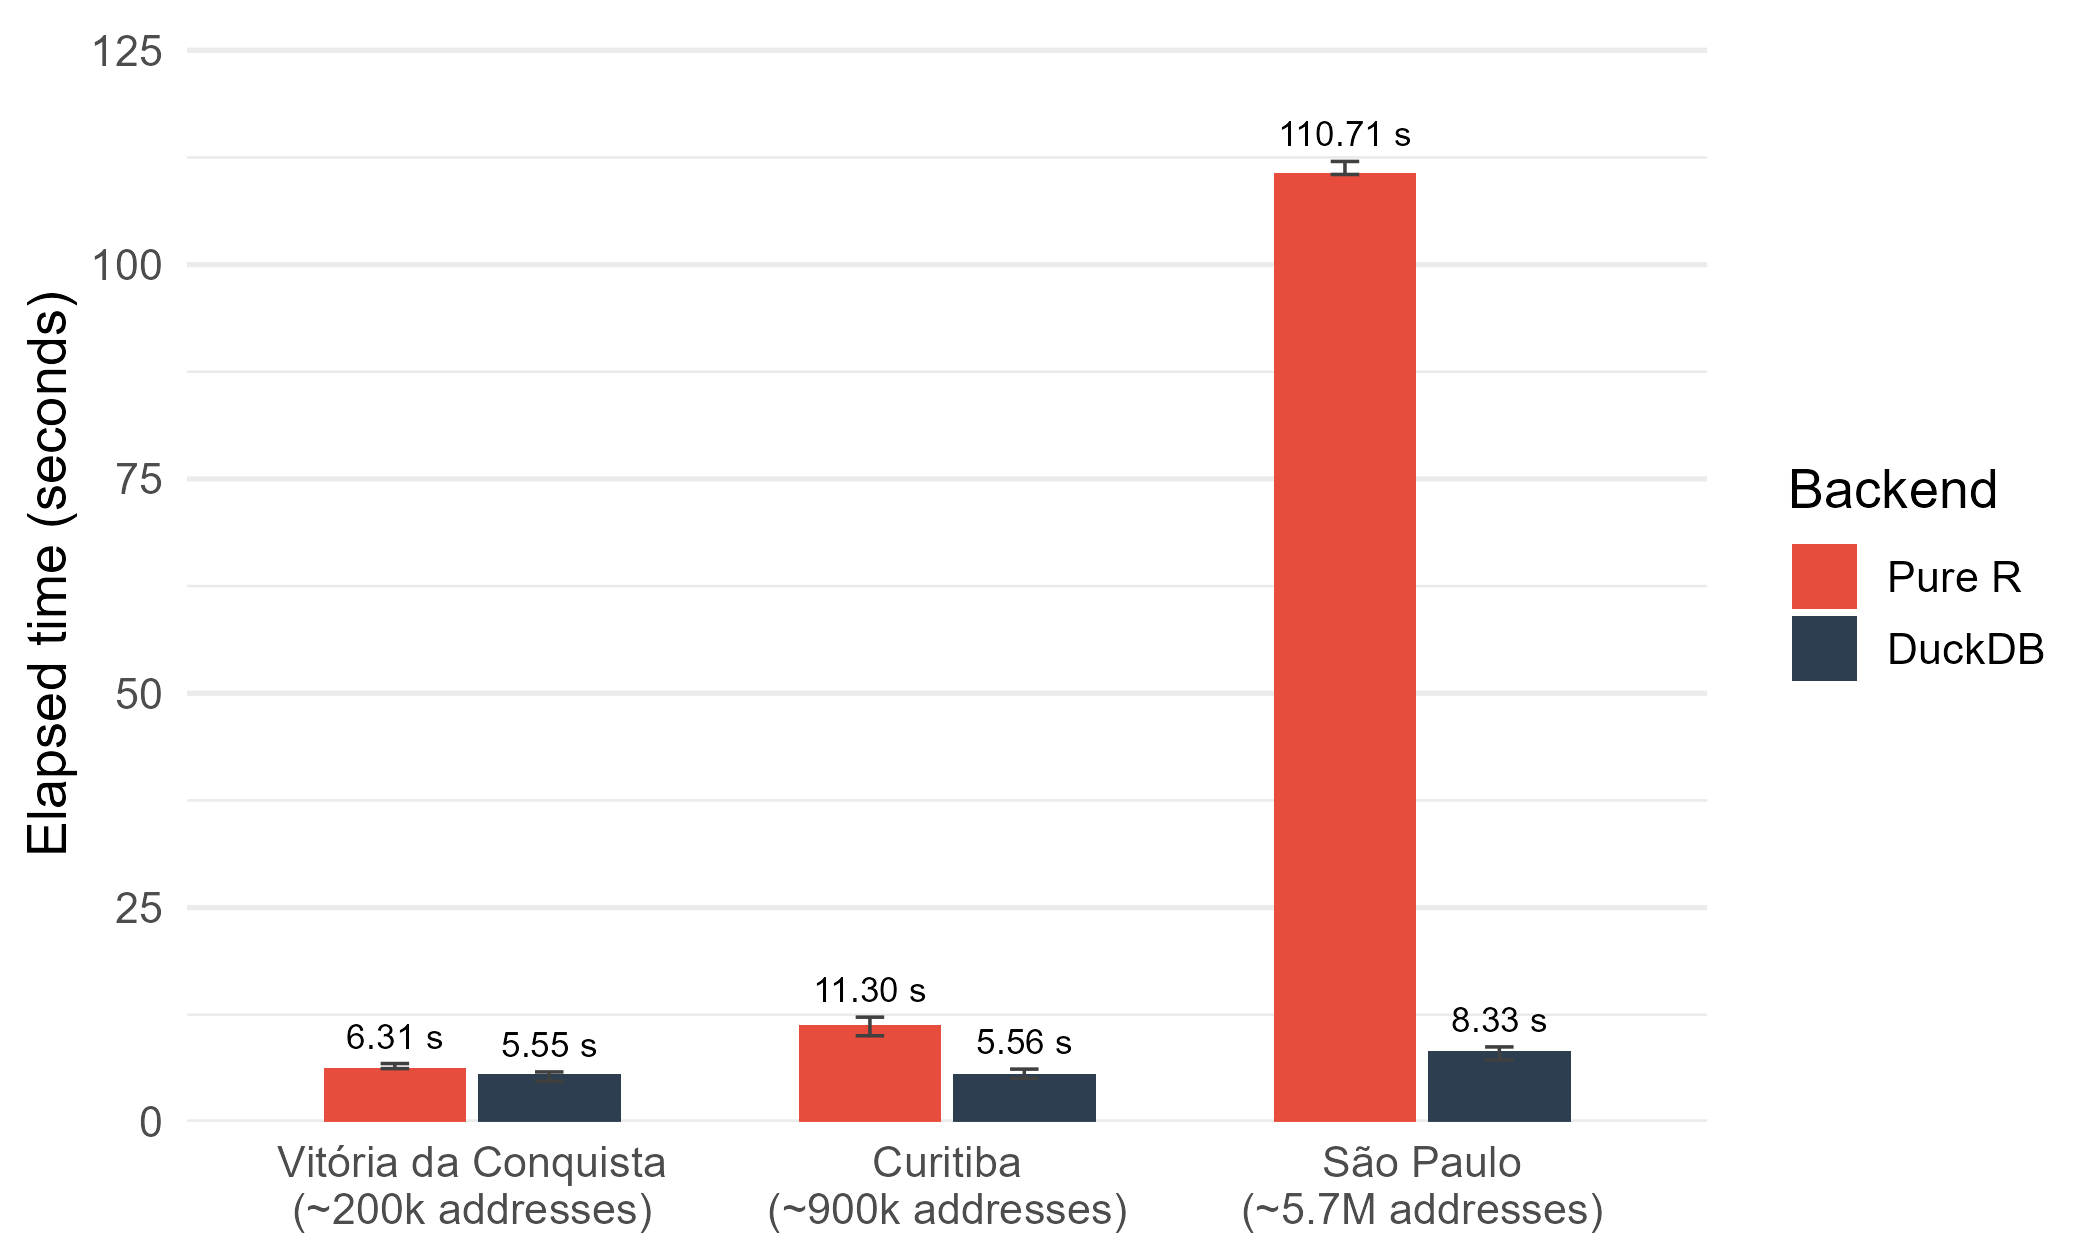
\includegraphics[width=0.7\linewidth,alt={Grouped bar chart comparing elapsed time in seconds for cnefe_counts() at H3 resolution 8 across three municipalities of increasing size: Vitória da Conquista-BA (roughly 200,000 addresses), Curitiba-PR (roughly 900,000 addresses), and São Paulo-SP (roughly 5.7 million addresses). For each municipality, two bars represent the DuckDB and pure-R backends; the DuckDB bar is shorter for larger municipalities, indicating increasing speedup with dataset size.}]{figures/bench-cities} 

}

\caption{Elapsed time (s) for \texttt{cnefe\_counts()} at H3 resolution~8, by municipality size, comparing the DuckDB and pure-R backends.}\label{fig:fig-bench-cities}
\end{figure}

Figure \ref{fig:fig-bench-h3} shows results for Curitiba-PR across
three H3 resolutions. The DuckDB speedup is 2.17× at resolution 7, 2.39×
at resolution 9, and 1.17× at resolution 11. At finer resolutions (higher
cell counts), the point-to-cell indexing dominates the total runtime, and
both backends ultimately delegate it to the same underlying H3 C library,
so the relative DuckDB advantage shrinks.

\begin{figure}

{\centering 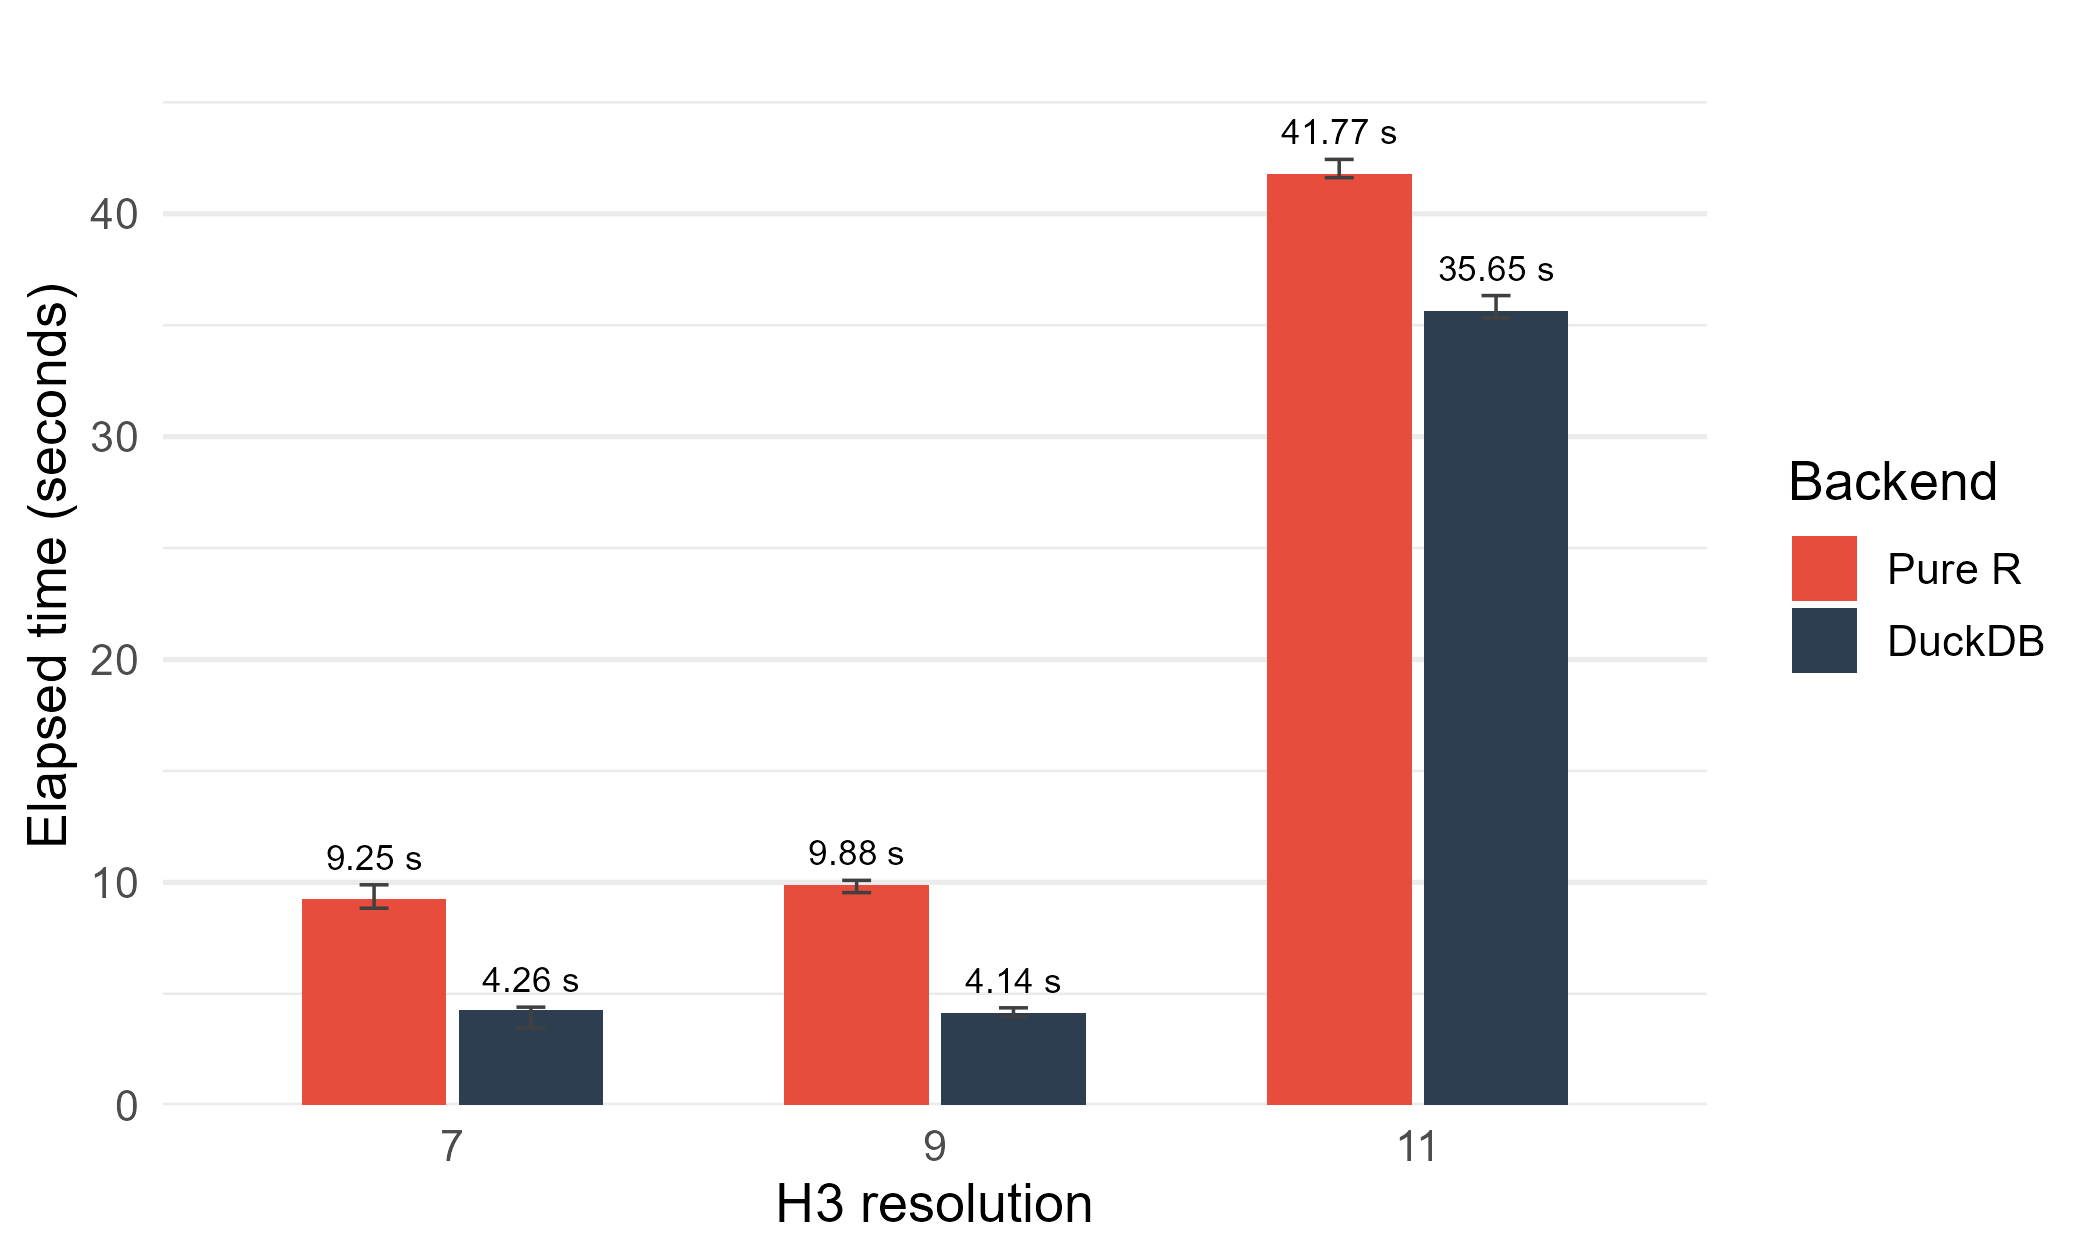
\includegraphics[width=0.7\linewidth,alt={Grouped bar chart comparing elapsed time in seconds for cnefe_counts() on Curitiba-PR across three H3 resolutions: 7 (coarse), 9 (medium), and 11 (fine). For each resolution, two bars represent the DuckDB and pure-R backends; the DuckDB speedup decreases at finer resolutions as H3 indexing cost becomes dominant.}]{figures/bench-h3} 

}

\caption{Elapsed time (s) for \texttt{cnefe\_counts()} on Curitiba-PR, by H3 resolution.}\label{fig:fig-bench-h3}
\end{figure}

\subsection{Memory}\label{memory}

Figure \ref{fig:fig-bench-memory} reports peak memory for the same
comparison, and it runs opposite to the intuition that an in-process
analytical database is the memory-hungry option. DuckDB stays nearly
flat across a 28-fold increase in input, rising only from 0.46 GB on
Vitória da Conquista-BA to 0.70 GB on São Paulo-SP, because it streams
and aggregates rather than materialising the address table. The pure-R
backend holds the filtered table in R memory, so its footprint scales
with the input and reaches 9.03 GB on São Paulo-SP, 12.8 times the
DuckDB figure.

\begin{figure}

{\centering 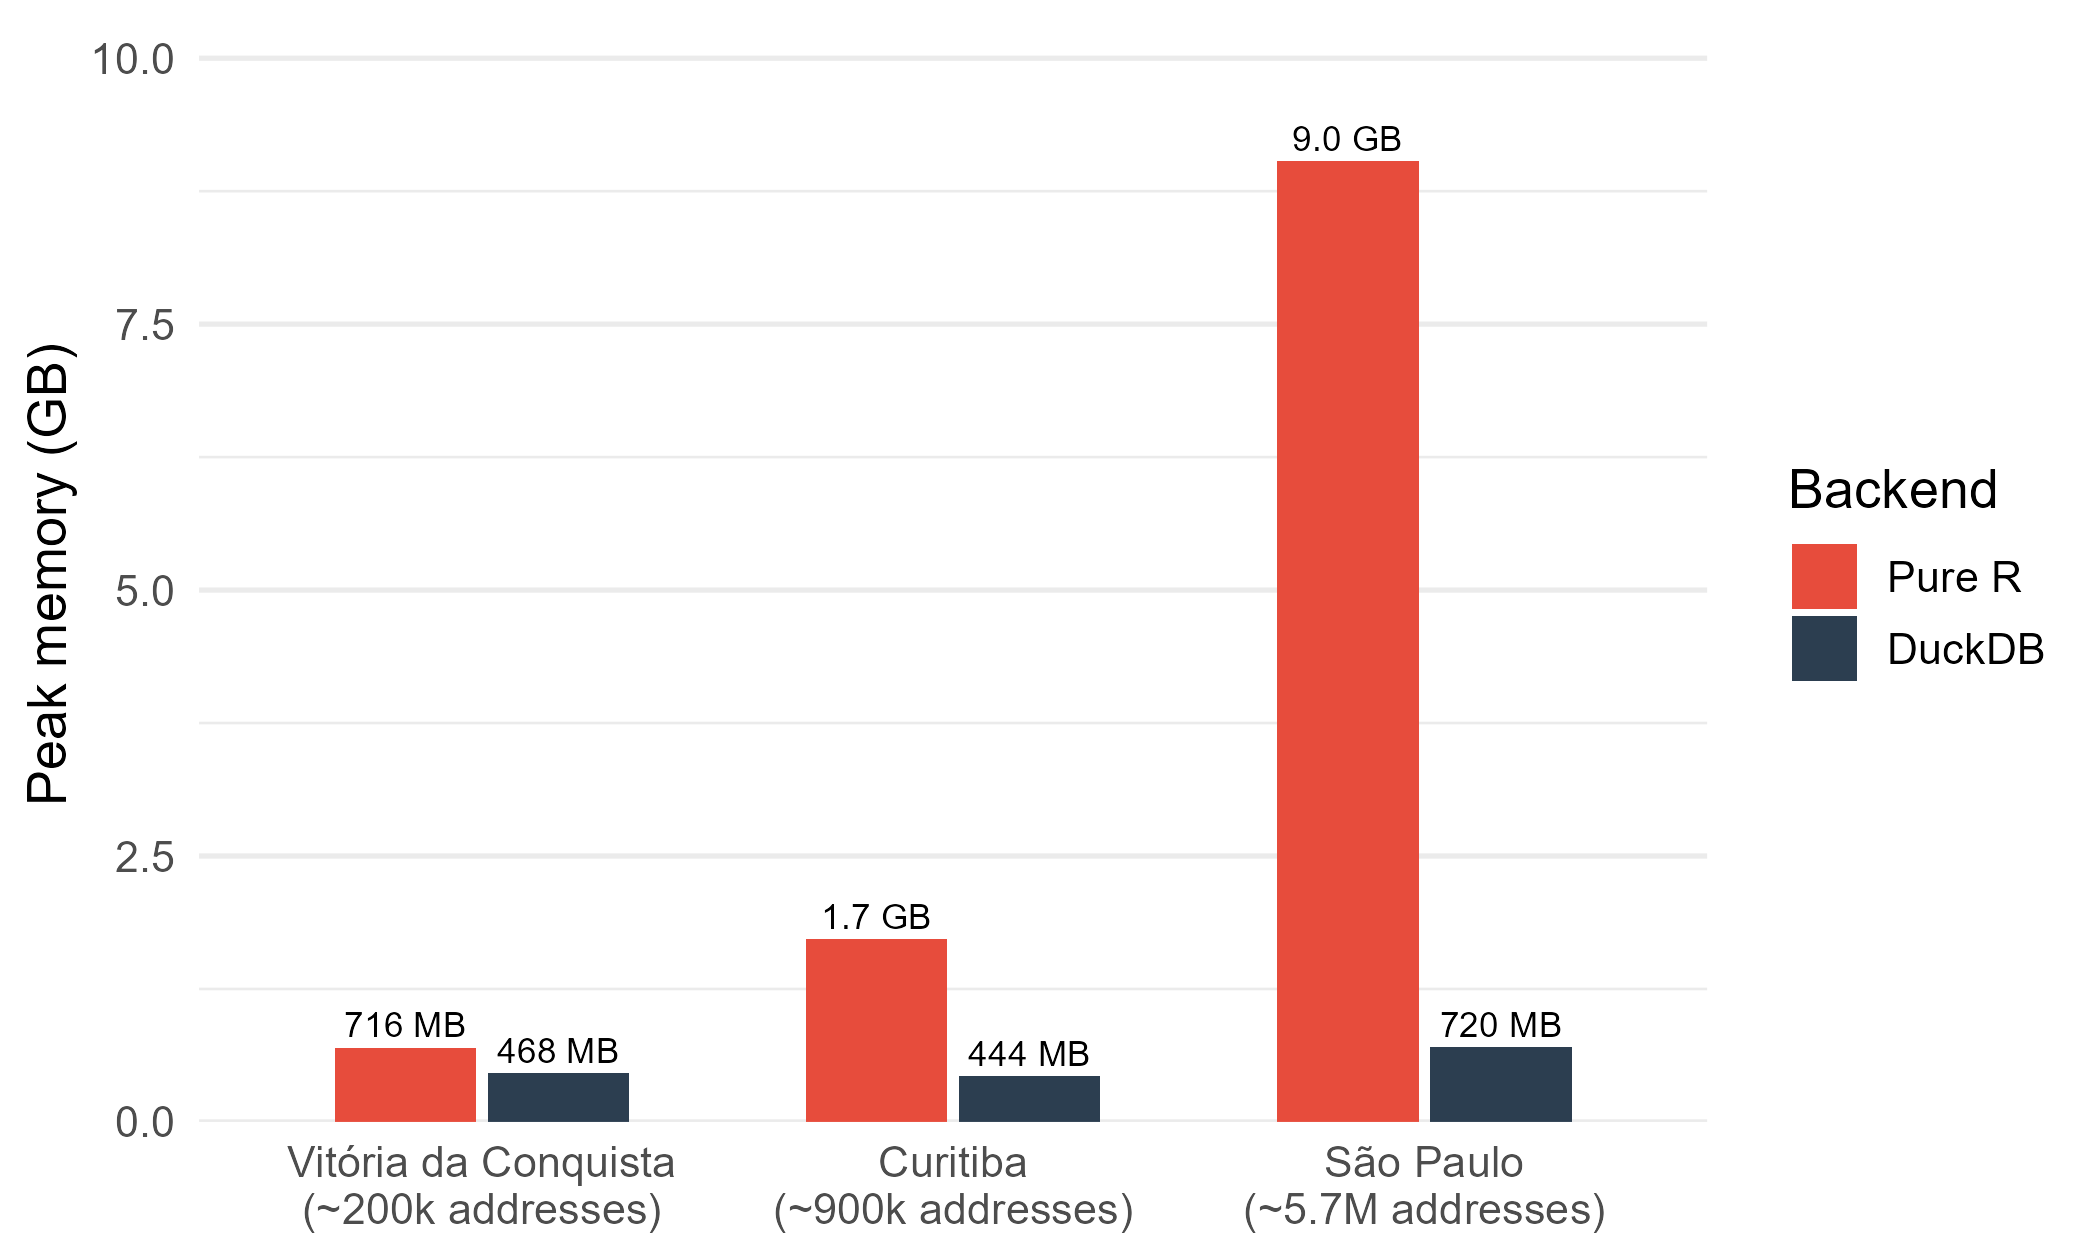
\includegraphics[width=0.7\linewidth,alt={Grouped bar chart comparing peak memory in gigabytes for cnefe_counts() at H3 resolution 8 across three municipalities of increasing size. For each municipality, two bars represent the DuckDB and pure-R backends; the DuckDB bars stay nearly constant at or below 0.7 GB while the pure-R bars grow with municipality size, reaching about 9 GB for São Paulo.}]{figures/bench-memory} 

}

\caption{Peak memory (GB) for \texttt{cnefe\_counts()} at H3 resolution~8, by municipality size, comparing the DuckDB and pure-R backends.}\label{fig:fig-bench-memory}
\end{figure}

This separates two constraints that were previously treated as one. The
pure-R backend is the appropriate choice when DuckDB extensions cannot
be installed, such as on some restricted computing clusters, which is
the case it was written for, and it is the wrong choice when the binding
constraint is memory. DuckDB sets \texttt{memory\_limit} to 80\% of installed RAM
by default, so it asks for less on a smaller machine, and a query that
exceeds the limit spills to a temporary directory instead of failing.
The budget can also be set explicitly:

\begin{verbatim}
options(cnefetools.duckdb_config = list(threads = 4, memory_limit = "4GB"))
\end{verbatim}

\subsection{Other heavy functions}\label{other-heavy-functions}

\texttt{compute\_lumi()} performs the same scan, the same H3 assignment and the
same grouped aggregation as \texttt{cnefe\_counts()}, and then adds arithmetic
that runs once per output cell rather than once per address, which on
São Paulo-SP is roughly four orders of magnitude fewer operations.
Measured at H3 resolution 8, the ratio between the two functions stays
between 0.95 and 1.19 across all three municipalities and both backends,
with no trend in input size, so the indices are effectively free relative
to the aggregation that produces them. We report the equivalence rather
than plotting the same curve twice.

The dasymetric interpolation functions behave differently and are
reported separately in Table \ref{tab:tab-bench-tracts}. They overlay
the full CNEFE point set against census tract polygons and download the
tract attributes for the whole state, and they run only on DuckDB. Two
features are worth noting. Their cost does not track address count:
Vitória da Conquista-BA is slower than Curitiba-PR despite being four
and a half times smaller, because at that size the runtime is dominated
by loading the state's census tract Parquet file, and Bahia's is more
than twice the size of Paraná's. In addition, \texttt{tracts\_to\_polygon()} is
the most memory-hungry path in the package, reaching 4.28 GB on São
Paulo-SP, because an overlay against arbitrary user polygons cannot use
the H3 shortcut.

\begin{longtable}[]{@{}
  >{\raggedright\arraybackslash}p{(\linewidth - 4\tabcolsep) * \real{0.4225}}
  >{\centering\arraybackslash}p{(\linewidth - 4\tabcolsep) * \real{0.2535}}
  >{\centering\arraybackslash}p{(\linewidth - 4\tabcolsep) * \real{0.3239}}@{}}
\caption{\label{tab:tab-bench-tracts} Median elapsed time and peak memory for the
dasymetric interpolation functions, at H3 resolution 9 on the DuckDB
backend.}\tabularnewline
\toprule\noalign{}
\begin{minipage}[b]{\linewidth}\raggedright
Municipality
\end{minipage} & \begin{minipage}[b]{\linewidth}\centering
\texttt{tracts\_to\_h3()}
\end{minipage} & \begin{minipage}[b]{\linewidth}\centering
\texttt{tracts\_to\_polygon()}
\end{minipage} \\
\midrule\noalign{}
\endfirsthead
\toprule\noalign{}
\begin{minipage}[b]{\linewidth}\raggedright
Municipality
\end{minipage} & \begin{minipage}[b]{\linewidth}\centering
\texttt{tracts\_to\_h3()}
\end{minipage} & \begin{minipage}[b]{\linewidth}\centering
\texttt{tracts\_to\_polygon()}
\end{minipage} \\
\midrule\noalign{}
\endhead
\bottomrule\noalign{}
\endlastfoot
Vitória da Conquista-BA (\textasciitilde200k) & 9.77 s, 0.66 GB & 7.27 s, 0.80 GB \\
Curitiba-PR (\textasciitilde900k) & 6.91 s, 0.61 GB & 5.25 s, 1.09 GB \\
São Paulo-SP (\textasciitilde5.7M) & 15.65 s, 1.93 GB & 15.53 s, 4.28 GB \\
\end{longtable}

\subsection{Constrained resources}\label{constrained-resources}

Table \ref{tab:tab-bench-modest} reports the largest municipality
re-run with DuckDB held to four threads and a 4 GB memory limit, which
the \texttt{cnefetools.duckdb\_config} option makes settable. São Paulo-SP
aggregates in about seven seconds within that budget, 26\% slower than on
the full machine while using 36\% less memory, and the dasymetric
interpolation costs 34\% more time, so neither degrades sharply as the
envelope tightens.

\begin{longtable}[]{@{}lcc@{}}
\caption{\label{tab:tab-bench-modest} Median elapsed time and peak memory on São
Paulo-SP under a constrained DuckDB configuration, against the same
calls with the machine's full resources.}\tabularnewline
\toprule\noalign{}
São Paulo-SP (\textasciitilde5.7M addresses) & full machine & 4 threads, 4 GB \\
\midrule\noalign{}
\endfirsthead
\toprule\noalign{}
São Paulo-SP (\textasciitilde5.7M addresses) & full machine & 4 threads, 4 GB \\
\midrule\noalign{}
\endhead
\bottomrule\noalign{}
\endlastfoot
\texttt{cnefe\_counts()} & 5.58 s, 0.70 GB & 7.01 s, 0.45 GB \\
\texttt{tracts\_to\_h3()} & 15.65 s, 1.93 GB & 20.93 s, 1.75 GB \\
\end{longtable}

This shows that the package works within a small resource envelope, but
it is not a substitute for measuring on older hardware, since the
storage, the RAM speed, the CPU generation and the operating system are
all unchanged. A genuinely older machine would do worse, particularly on
the initial read, which is bound by input and output rather than by
computation and which limiting the thread count does not reproduce. The
machine specification is reported above so that readers can scale
expectations accordingly.

For most users, the default DuckDB backend is recommended, on both time
and memory. The pure-R backend (\texttt{backend\ =\ "r"}) remains available for
environments where DuckDB extensions cannot be installed.

\section{Summary}\label{summary}

\CRANpkg{cnefetools} makes the 2022 Brazilian CNEFE address dataset
accessible and analytically useful from R. Its principal contributions
are:

\begin{enumerate}
\def\labelenumi{\arabic{enumi}.}
\tightlist
\item
  \textbf{Data access}: a pre-built municipality index and persistent
  caching layer that abstract away the FTP structure and eliminate
  repeated downloads.
\item
  \textbf{Address aggregation}: flexible aggregation of address counts to
  H3 hexagonal grids or arbitrary polygons, supporting both a fast
  DuckDB backend and a portable pure-R fallback.
\item
  \textbf{Land use mix indices}: a complete implementation of six
  established and novel LUM indices, including the directional,
  globally referenced BGBI.
\item
  \textbf{Dasymetric interpolation}: tract-to-hexagon and tract-to-polygon
  redistribution of census variables using CNEFE dwelling points as
  ancillary data, with per-variable allocation diagnostics.
\item
  \textbf{DuckDB dual-backend}: a performance architecture that streams the
  cached gzipped CSV, assigns H3 cells and performs spatial joins
  entirely within an in-process DuckDB engine. Its advantage grows
  with dataset size, exceeding fifteenfold on the largest
  municipality, where its peak memory is also more than twelve times
  smaller than the pure-R backend's.
\end{enumerate}

The package also has some limitations. First, data access depends on
IBGE, and that dependency carries two different risks. The FTP server
may be unavailable, which the cache mitigates, since a municipality that
has been downloaded once keeps working without a connection. The terms
of access may also change, since publishing individual geocoded address
points for a whole country is unusually granular for a national
statistical product, and a future review could put the CNEFE behind authentication,
aggregation or a licence, which no caching strategy can mitigate. What
the package offers against that risk is that \texttt{read\_cnefe(file\ =\ ...)}
reads a file obtained through another channel without going through the
download, although the analytical functions still retrieve their data
through the cache and would need the same option to work in that
situation. Second, although the package supports aggregation to H3 grids
and user-supplied polygons, its core analytical workflows are organised
around municipality-specific inputs, which limits analyses that span
multiple municipalities or other cross-boundary study regions. Third,
the land use mix implementation is restricted to a binary residential
versus non-residential formulation, even though the underlying CNEFE
classification distinguishes a richer set of address types.

The second limitation matters most for research questions posed at the
scale of a metropolitan region. Analyses of that kind are achievable
today by iterating the relevant function over a vector of municipality
codes and combining the results, and \citet{pedreirajr2026} gives a worked
example applying exactly that pattern across the 39 municipalities of
the São Paulo metropolitan region. Two caveats apply when doing so. The
H3 grid built by \texttt{cnefe\_counts()} and \texttt{compute\_lumi()} is derived from
each municipality's own boundary, and cells are selected by whether
their centre falls inside it, so a cell straddling a shared border
belongs to exactly one of the two municipalities and its counts reflect
only that municipality's addresses. The citywide residential share \(P\)
that \texttt{compute\_lumi()} uses as its reference is likewise computed per
municipality, which is the intended behaviour but means that indices
defined against it are not directly comparable across municipalities
without recomputing the baseline for the wider area.

The third limitation matters for questions in which the kind of
non-residential use is the point. The binary split places agricultural
establishments (type 3), which make up 3.7\% of all addresses and are
qualitatively different from urban uses, in the same group as schools
and hospitals, and it merges other-purpose establishments (type 6), a
heterogeneous category that includes commerce and services and makes up
10.5\% of addresses, with educational, health and religious ones. A
study of urban health that needs to separate commercial from
institutional uses, for example, cannot do so with these indices. For
such questions, the counts returned by \texttt{cnefe\_counts()} keep all eight
address types and can feed a multi-category index directly.

A related design choice concerns what \texttt{read\_cnefe()} returns. It
returns an Arrow table or an \texttt{sf} object held in memory, rather than a
lazy DuckDB relation that would be evaluated only when queried. A lazy
relation is valid only while its database connection is open, so
returning one would mean keeping a connection alive after the function
returns, whereas every function in the package closes its connection
before returning, which guarantees that no connection is left open after
an error or an interruption. For a municipality too large to hold in
memory comfortably, the better route is to export it to Parquet with
\texttt{cnefe\_export()} and query the file lazily with \texttt{arrow::open\_dataset()}
or DuckDB.

Future development will focus on reducing these constraints. One
priority is to provide access to preprocessed remote Parquet assets for
CNEFE data, reducing reliance on the IBGE FTP infrastructure and
improving robustness and read performance. Another is to further
leverage DuckDB's spatial extension to support arbitrary polygon layers
and hexagonal grids that are not restricted to municipal boundaries,
while handling the necessary municipal CNEFE files internally. A third
direction is to expand the land use mix module with additional indices
and formulations that exploit the multi-category structure of CNEFE,
moving beyond the current binary residential/non-residential approach.

\CRANpkg{cnefetools} is available on CRAN and its development version on
GitHub (\url{https://github.com/pedreirajr/cnefetools}). Documentation and
pre-rendered vignettes are available at
\url{https://pedreirajr.github.io/cnefetools/}.

\bibliography{cnefetools.bib}

\address{%
Jorge Ubirajara Pedreira Junior\\
Universidade Federal da Bahia\\%
Escola Politécnica\\ Salvador, Bahia, Brazil\\
%
\url{https://pedreirajr.github.io/website/}\\%
\textit{ORCiD: \href{https://orcid.org/0000-0002-8243-5395}{0000-0002-8243-5395}}\\%
\href{mailto:jorge.ubirajara@ufba.br}{\nolinkurl{jorge.ubirajara@ufba.br}}%
}

\address{%
Bruno Henrique Mioto Stabile\\
Universidade Estadual de Maringá\\%
Programa de Pós-Graduação em Ecologia de Ambientes Aquáticos Continentais (PEA-UEM)\\ Maringá, Paraná, Brazil\\
%
%
\textit{ORCiD: \href{https://orcid.org/0000-0002-3524-537X}{0000-0002-3524-537X}}\\%
\href{mailto:bhmstabile@gmail.com}{\nolinkurl{bhmstabile@gmail.com}}%
}
